\documentclass[
    chapter=TITLE,
    12pt, 		% Tamanho da fonte
    openright,% Capítulos começam em pág. ímpar (insere página vazia caso preciso)
    oneside, 	% Para impressão somente verso. Oposto a impressão em verso e anverso
    hidelinks,
    a4paper, 	% Tamanho do papel
    english, 	% Idioma adicional para hifenização
    brazil 		% o último idioma é o principal do documento
    ]{abntex2}

\renewcommand{\theequation}{\arabic{equation}}  
\usepackage[utf8]{inputenc}
\usepackage{tikz}
\usepackage{wrapfig}
\usetikzlibrary{calc}
\usepackage{lipsum} 	% para geração de dummy text
\usepackage{multirow}
\usepackage{algpseudocode}
\usepackage{algorithm}
\usepackage{svg}

\usepackage{pdflscape} %para poder rotacionar a página
%\usepackage[table,xcdraw]{xcolor}
\PassOptionsToPackage{table,xcdraw}{xcolor}

% Pacotes
%% Sumário
%\usepackage{tocloft}
\setlength{\cftbeforechapterskip}{0pt}


%% Referência
%\usepackage[hyphenbreaks]{breakurl}
% \usepackage[alf]{abntex2cite}
% \usepackage[alf,abnt-etal-list=0,abnt-etal-cite=3]{abntex2cite} %et al qnd cita apenas
\usepackage[alf,bibjustif,abnt-etal-cite=2]{abntex2cite} %et al na referência tbm e justificada
\usepackage{hyperref}

%\usepackage[hyphenbreaks]{breakurl}
%\usepackage[num,overcite,'-emphasize=em]{abntex2cite}

%% Codificação
\usepackage[T1]{fontenc} 	% Codificação de saída

%% Fonte
\usepackage{times} 			% Times New Roman

\usepackage{lastpage} 		% Usado pela Ficha catalográfica
\usepackage{indentfirst} 	% Indenta o primeiro parágrafo de cada seção.
\usepackage{color} 				% Controle das cores
\usepackage{microtype} 		% Para melhorias de justificação
\usepackage{lscape} 			% Permite a criação de conteúdo em modo paisagem
\usepackage{hyperref} 		% Criação de links
\usepackage{etoolbox}

%% Tabelas
\usepackage{multirow}

%% Equação
\usepackage{amsmath}

%% Sumário
\usepackage{textcase}

%% Imagens
\usepackage{graphicx} % Inclusão de gráficos

%% Tamanho e alinhamento das legendas
\usepackage[
	singlelinecheck=false,
	justification=justified,
	font=footnotesize
	]
	{caption}
\usepackage{pdfpages}


\usepackage{listings}

\usepackage{url}
\renewcommand{\UrlLeft}{}  % Remove o símbolo de abertura (por padrão é `<`)
\renewcommand{\UrlRight}{} % Remove o símbolo de fechamento (por padrão é `>`)


%Nome do autor
% Especificidades para a entrada de autor pessoal: – sobrenome com indicativo de parentesco
% Quando o autor é brasileiro, trate o grau de parentesco como parte do sobrenome.
% Exemplo: Autor: Luís Fernando Carvalho Neto - Entrada: CARVALHO NETO, L. F.
\autor{Thamires Ramos dos Santos}
\newcommand{\entradaAutor}{DOS SANTOS, Thamires Ramos} % Sem ponto no final

% Titulo do trabalho
\titulo{O papel da engenharia da computação na prevenção de acidentes em barragens de rejeitos} %Título do trabalho
\newcommand{\englishTitle}{The role of computer engineering in preventing tailings dam accidents} %Título do trabalho em inglês
\data{\today}			%Ano de publicação
\local{Nova Friburgo}	%Local

%% Membros da banca
\newcommand{\membrobancaA}{Prof. Dr. Banca 1}
\newcommand{\intituicaoBancaA}{Instituto Politécnico - UERJ}

\newcommand{\membrobancaB}{Prof. Dr. Banca 2}
\newcommand{\intituicaoBancaB}{Instituto Politécnico - UERJ}


\renewcommand{\familydefault} {\sfdefault} 			% Seta fonte default
\makepagestyle	{abntheadings}
\makeevenhead {abntheadings} {\ABNTEXfontereduzida\thepage} {} {\ABNTEXfontereduzida\textit\leftmark}
\makeoddhead {abntheadings} {} {} {\ABNTEXfontereduzida\thepage}
\makeheadrule {abntheadings} {0pt} {\normalrulethickness}

\makepagestyle {abntchapfirst} 
\makeoddhead {abntchapfirst} {} {} {\ABNTEXfontereduzida\thepage}

\providecommand{\imprimirmembrobancaA}{}
\providecommand{\imprimirmembrobancaAinst}{}
\providecommand{\imprimirmembrobancaB}{\membrobancaB}
\providecommand{\imprimirmembrobancaBinst}{}
\providecommand{\imprimirmembrobancaC}{\membrobancaC}
\providecommand{\imprimirmembrobancaCinst}{}


%\renewcommand{\membrobancaA}[2][\imprimirinstituicao]{\renewcommand{\imprimirmembrobancaA}{#2}\renewcommand{\imprimirmembrobancaAinst}{#1}}
%\renewcommand{\membrobancaB}[2][\imprimirinstituicao]{\renewcommand{\imprimirmembrobancaB}{#2}\renewcommand{\imprimirmembrobancaBinst}{#1}}
%\renewcommand{\membrobancaC}[2][\imprimirinstituicao]{\renewcommand{\imprimirmembrobancaC}{#2}\renewcommand{\imprimirmembrobancaCinst}{#1}}

%\newcommand{\imprimirmeOrientadorinst}{\imprimirinstituicao}
%\newcommand{\imprimirmeCoorientadorinst}{\imprimirinstituicao}

%% Natureza do trabalho
\providecommand{\imprimirnaturezatrabalho}{}\newcommand{\naturezatrabalho}[1]{\renewcommand{\imprimirnaturezatrabalho}{#1}}


%% Redefinir resumo
\renewenvironment{resumo}[1][\resumoname]{\pretextualchapter{#1}}{\PRIVATEclearpageifneeded}

%% Redefinir dedicatória
\renewenvironment{dedicatoria}[1][]{\ifthenelse{\equal{#1}{}}{\PRIVATEbookmarkthis{\dedicatorianame}}{\preamblealchapter{#1}}\vspace*{\fill}}{}

\renewenvironment{epigrafe}[1][]{\ifthenelse{\equal{#1}{}}{\PRIVATEbookmarkthis{\epigraphname}}{\pretextualchapter{#1}}\vspace*{\fill}}{}

%% Comando para inserir sigla
\newcommand{\sigla}[2][]{\item[#1] \textit{#2}}


%% Comando para inserir simbolo
%\newcommand{\simbolo}[2][]{
%	\item[#1] \textit{#2}
%}

%% Redefinição da formatação do \chapter
\renewcommand{\ABNTEXchapterfont}{\normalfont\fontseries{b}\selectfont}
\renewcommand{\ABNTEXchapterfontsize}{\normalsize}
\renewcommand{\ABNTEXpartfont}{\fontseries{b}\selectfont\selectfont}
\renewcommand{\ABNTEXpartfontsize}{\normalsize}
\renewcommand{\ABNTEXsectionfont}{\normalfont\selectfont} %\fontseries{b}
\renewcommand{\ABNTEXsectionfontsize}{\normalsize}
\renewcommand{\ABNTEXsubsectionfont}{\normalfont}
\renewcommand{\ABNTEXsubsectionfontsize}{\normalsize}
\renewcommand{\ABNTEXsubsubsectionfont}{\normalfont}
\renewcommand{\ABNTEXsubsubsectionfontsize}{\normalsize}
\renewcommand{\ABNTEXsubsubsubsectionfont}{\normalfont}
\renewcommand{\ABNTEXsubsubsubsectionfontsize}{\normalsize}
%\renewcommand{\ABNTEXsubsubsectionfont}{\normalfont\fontseries{b}\selectfont}
%\renewcommand{\ABNTEXsubsubsectionfontsize}{\normalsize}
%\renewcommand{\ABNTEXsubsubsubsectionfont}{\normalfont\itshape\selectfont}
%\renewcommand{\ABNTEXsubsubsubsectionfontsize}{\normalsize}



%% Redefinição da formatação de Parágrafos 
\setlength{\parindent}{1.3cm}
\setlength{\parskip}{0cm}



%% Sumário
\makeatletter
\addtocontents{toc}{\protect\renewcommand{\protect\cftchapterleader}{\normalsize\normalfont\protect\cftdotfill{\protect\cftdotsep}}}
\renewcommand{\cftchapterpresnum}{\normalfont} % Numeração do capítulo não ficar em negrito
\renewcommand{\cftchapterpagefont}{\normalfont} % Páginas do capítulo não ficar em negrito
\renewcommand*{\cftchapterfont}{\normalfont\bfseries} % Título do capítulo em negrito
\renewcommand{\chapnumfont}{\normalfont\normalsize}
\renewcommand*{\cftsectionfont}{\normalfont} %\fontseries{b}
\renewcommand*{\cftsubsectionfont}{\normalfont}
\renewcommand*{\cftsubsubsectionfont}{\normalfont}
\renewcommand*{\cftsubsubsubsectionfont}{\normalfont}
\renewcommand*{\cftparagraphfont}{\normalfont} %\itshape

%% Forca underline na secao terciaria
\newcommand{\tmpsubsection}[1]{}
\let\tmpsubsection=\subsection
\renewcommand{\subsection}[1]{\tmpsubsection{\underline{#1}}}

%% Forca underline na secao secundaroa
\newcommand{\tmpsection}[1]{}
\let\tmpsection=\section
\renewcommand{\section}[1]{\tmpsection{\textbf{#1}}}
\makeatother

%% Tornar as seções secundários com fonte em maiúscula
%\makeatletter
%\let\oldcontentsline\contentsline
%\def\contentsline#1#2{%
%  \expandafter\ifx\csname l@#1\endcsname\l@section
%    \expandafter\@firstoftwo
%  \else
%    \expandafter\@secondoftwo
%  \fi
%  {%
%    \oldcontentsline{#1}{\MakeTextUppercase{#2}}%
%  }{%
%    \oldcontentsline{#1}{#2}%
%  }%
%}
%\makeatother

%% Tornar a entrada "Referências" com fonte em maiúscula
%%\addto\captionsbrazil{
%%    \renewcommand{\bibname}{REFER\^ENCIAS}
%%}
% Legendas
\makeatletter
\patchcmd{\caption@@@make}
{\ifcaption@star}
{\ifcaption@star\small}
{}{}
\makeatother


\graphicspath{ {figures/} }

\preambulo{
Trabalho de conclusão de curso apresentado como pré-requisito para obtenção do título de Engenheiro de Computação, ao Departamento de Modelagem Computacional, do Instituto Politécnico, da Universidade do Estado do Rio de Janeiro.
}

\orientador{Prof. Edgard Poiate Junior.}
\tipotrabalho{monografia}		%Define as configurações do arquivo

\begin{document}
    \newpage
    \pagenumbering{arabic}
	
    %Capa
	\renewcommand{\imprimircapa}{%
	\begin{center}
		\begin{tikzpicture}[remember picture, overlay]
		\draw[line width = 4pt] ($(current page.north west) + (20mm, -20mm)$) rectangle ($(current page.south east) + (-10mm,10mm)$);
		\draw[line width = 1pt] ($(current page.north west) + (21.5mm,-21.5mm)$) rectangle ($(current page.south east) + (-11.5mm,11.5mm)$);
		\end{tikzpicture}
		\begin{capa}            
            \begin{minipage}{\linewidth}                
    			\begin{minipage}{0.23\linewidth}
                    \centering
    				
\includegraphics[width=2.5cm]{uerj}
                \end{minipage}%
                \hfill
                \begin{minipage}{0.51\linewidth}
    				\begin{center}
    					\textbf{UNIVERSIDADE DO ESTADO DO \\ RIO DE JANEIRO}\\
    					\noindent\rule{7cm}{0.4pt}\\
    					\textbf{INSTITUTO POLITÉCNICO \\ GRADUAÇÃO EM ENGENHARIA \\DE COMPUTAÇÃO}\\
    				\end{center}
    			\end{minipage}
       			\hfill
                \begin{minipage}{0.23\linewidth}                
    				
\includegraphics[width=3.5cm]{iprj}
                    \vspace{1cm}
                \end{minipage}
            \end{minipage}
			\vspace*{4.5cm}
			\center
			\textbf{\large\imprimirautor}
			\vspace*{3cm}
			\begin{center}
				\textbf{\large\imprimirtitulo}
			\end{center}
			\vfill
			\textbf{
				\large\imprimirlocal
				\\	
				\large \the\year
			}
			\vspace*{1cm}
		\end{capa}
	\end{center}
}
\imprimircapa
	
	%Folha de rosto	
    \makeatletter
\renewcommand{\folhaderostocontent}{
	\begin{center}
		\begin{tikzpicture}[remember picture, overlay]
			\draw[line width = 4pt] ($(current page.north west) + (20mm, -20mm)$) rectangle ($(current page.south east) + (-10mm,10mm)$);
			\draw[line width = 1pt] ($(current page.north west) + (21.5mm,-21.5mm)$) rectangle ($(current page.south east) + (-11.5mm,11.5mm)$);
		\end{tikzpicture}

        \begin{minipage}{\linewidth}                
            \begin{minipage}{0.23\linewidth}
                \centering
                
\includegraphics[width=2.5cm]{uerj}
            \end{minipage}%
            \hfill
            \begin{minipage}{0.51\linewidth}
                \begin{center}
                    \textbf{UNIVERSIDADE DO ESTADO DO \\ RIO DE JANEIRO}\\
                    \noindent\rule{7cm}{0.4pt}\\
                    \textbf{INSTITUTO POLITÉCNICO \\ GRADUAÇÃO EM ENGENHARIA \\DE COMPUTAÇÃO}\\
                \end{center}
            \end{minipage}
            \hfill
            \begin{minipage}{0.23\linewidth}                
                
\includegraphics[width=3.5cm]{iprj}
                \vspace{1cm}
            \end{minipage}
        \end{minipage}
        
		\vspace*{2cm}
		\begin{center}
			{\imprimirautor}
			\vspace*{\fill}\vspace*{\fill}
			\begin{center}
				\textbf{\imprimirtitulo}
			\end{center}
			\vspace*{\fill}
			\abntex@ifnotempty{\imprimirpreambulo}{%
				\hspace{.45\textwidth}
				\begin{minipage}{.5\textwidth}
					\SingleSpacing
					\imprimirpreambulo
				\end{minipage}%
				\vspace*{2cm}
				\vspace*{\fill}
			}%
			{\abntex@ifnotempty{\imprimirinstituicao}{\imprimirinstituicao\vspace*{\fill}}}
			\begin{flushleft}
				{\imprimirorientadorRotulo~\imprimirorientador\par}
			\end{flushleft}
			\abntex@ifnotempty{\imprimircoorientador}{%
				{\imprimircoorientadorRotulo~\imprimircoorientador}%
			}%            
			\vspace*{\fill}
			{\imprimirlocal}
			\par
			{\the\year}
			\vspace*{1cm}
		\end{center}	
	\end{center}
}
\makeatother
	\imprimirfolhaderosto

	%Catalogação Biblioteca
	\newcommand{\imprimircatalogacao}{%
    \noindent
    UNIVERSIDADE DO ESTADO DO RIO DE JANEIRO\\
    INSTITUTO POLITÉCNICO\\
    CURSO DE ENGENHARIA DE COMPUTAÇÃO
    
    \vspace{1cm}
    \noindent
    Reitora: Gulnar Azevedo e Silva\\
    Vice-reitor: Bruno Rêgo Deusdará Rodrigues\\
    Diretor do Instituto Politécnico: Lucas Venâncio Pires de Carvalho Lima\\
    Coordenador de Curso: Rodrigo Lamblet Mafort
    
    \vspace{1cm}
    \noindent
    Banca Avaliadora Composta por: \imprimirorientador~(Orientador)\\
    \hspace*{6.3cm}\membrobancaA\\
    \hspace*{6.3cm}\membrobancaB
    
    \vspace{0.5cm}
    \noindent
    \includegraphics[
        page=1,
        trim={4cm 3cm 0cm 18cm},
        clip,
        width=17cm,
        height=9cm  %era 10
    ]{FichaCatalográfica.pdf}
    %https://www.rsirius.uerj.br/servicos/elaboracao_ficha/instrucoes   gerar a sua
    %http://www.sirius.uerj.br/ficha/ficha104.php  preencher os dados
    
    \pagenumbering{gobble}
    \vspace{0.5cm}
    \noindent
    Endereço: UERJ - IPRJ\\
    \hspace*{2cm} CEP 28625-570 - Nova Friburgo - RJ - Brasil.
    
    \vspace{0.5cm}
    \noindent
    Este trabalho nos termos da legislação que resguarda os direitos autorais é considerado de propriedade da Universidade do Estado do Rio de Janeiro (UERJ). É permitida a transcrição parcial de partes do trabalho, ou mencioná-lo, para comentários e citações, desde que sem propósitos comerciais e que seja feita a referência bibliográfica completa.
    \begin{flushright}
        \assinatura{\imprimirautor}
    \end{flushright}
}

\imprimircatalogacao
\pagenumbering{arabic}
	
	%Folha de aprovação
	\newcommand{\imprimirfolhaaprovacao}{%
	\begin{folhadeaprovacao}
		\begin{center}
			%{\large{\imprimirautor}}\\[1cm]
            {\imprimirautor}\\[1cm]
			\vspace{2cm}
			%{\Large\bfseries\imprimirtitulo}
            {\bfseries\imprimirtitulo}
		\end{center}		
		\vspace{1cm}
		\hspace{.45\textwidth}
		\begin{minipage}{.5\textwidth}
			{\fontsize{12}{12}\selectfont{\imprimirpreambulo}}
		\end{minipage}%
		\\\\\\\\
		\vspace{1cm}
		Aprovado em XX de XXXXXXXX de 2025.\\
		\vspace{1.5cm}
		Banca examinadora:
		
		\assinatura{\flushleft{\imprimirorientador\vspace{0.2cm}\\Instituto Politécnico - UERJ}}
		\assinatura{\flushleft{\membrobancaA\\\intituicaoBancaA}}
        \assinatura{\flushleft{\membrobancaB\\\intituicaoBancaB}}
		\begin{center}
			\vfill
			%{\large\imprimirlocal}
			{\imprimirlocal}
			\vspace{0.2cm}
			\par
			%{\large\the\year}
			{\the\year}
		\end{center}		
	\end{folhadeaprovacao}
}

\imprimirfolhaaprovacao

	  %% Elemento opcional (Figura 10).
%% A palavra DEDICATÓRIA deve ser grafada em fonte 12, em
%% maiúsculas, negritada e centralizada na parte superior da folha.
%% O texto da dedicatória deve estar localizado na parte inferior da
%% folha, seguindo as regras gerais de apresentação gráfica.

\begin{epigrafe}[Dedicatória]

	Opcional. Aqui vai a dedicatória do trabalho. 

\end{epigrafe}
	%% A palavra AGRADECIMENTOS deve ser grafada em fonte 12,
%% em maiúsculas, negritada e centralizada na parte superior da folha.
%% O texto dos agradecimentos deve ser separado do título por duas
%% linhas em branco com espaçamento 1,5 e digitado de acordo as regras
%% gerais de apresentação gráfica.
%% Se houver necessidade, o texto pode continuar nas folhas seguin-
%% tes, sem incluir a palavra Agradecimentos.

\begin{agradecimentos}

Aqui vão os agradecimentos. 

\end{agradecimentos}
	  %% Elemento opcional.
%% É uma citação sem aspas – em fonte 12, estilo normal, com es-
%% paço 1,5 – seguida da indicação de autoria, grafada em fonte 12 e em
%% itálico.
%% O texto deve estar localizado no terço inferior da folha, com o ali-
%% nhamento livre, necessário à epígrafe.

\begin{epigrafe}
    \vspace*{\fill}
    \begin{flushright}
        Opcional. Citação de alguma frase ou texto conhecido. \\
        \textit{Aqui vai a autoria da frase ou texto}
    \end{flushright}
\end{epigrafe}

	%% 3.1.9 Resumo em língua portuguesa
%% Elemento obrigatório (Figura 14).
%% Consiste na apresentação sucinta dos pontos relevantes do texto,
%% em um único parágrafo. O resumo deve conter entre 150 e 500 pala-
%% vras e fornecer uma visão rápida e clara dos objetivos, da metodologia,
%% dos resultados e das conclusões do trabalho. Na elaboração do resumo,
%% deve-se usar o verbo na voz ativa, na terceira pessoa do singular.

%% Fonte -> TNR ou Arial, corpo 12.
%% A palavra RESUMO deve aparecer em letras maiúsculas
%% e em negrito.
%% O uso de itálico é permitido em palavras estrangeiras.
%% O uso de letras maiúsculas nas palavras-chave
%% restringe-se ao início da palavra, em nomes próprios
%% e siglas, se for o caso.

%% Alinhamento -> A palavra RESUMO deve estar localizada na margem
%% superior da folha e centralizada, e a referência, alinhada
%% à margem esquerda;
%% O alinhamento é justificado para o texto do resumo,
%% que inicia com parágrafo, e para as palavras-chave.

%% Espaçamento -> A palavra RESUMO deve ser separada da referência por
%% duas linhas em branco de 1,5;
%% Espaço 1 na referência e no resumo e, nas palavras-
%% chave, espaço 1,5.

%% Formato do papel,
%% orientação e margens -> Conforme especificado na seção 1.1.

%% Pontuação -> As palavras-chave devem ser separadas por ponto e
%% terminadas por ponto.

\begin{resumo}
\begin{SingleSpace}

\noindent
\begin{flushleft}
\entradaAutor{}. \textit{\imprimirtitulo}. \the\year. \pageref{LastPage} f. Trabalho de Conclusão de Curso (Graduação em Engenharia de Computação) - Instituto Politécnico, Universidade do Estado do Rio de Janeiro, Nova Friburgo, \the\year.
\end{flushleft}
\vspace{\onelineskip}

\setlength{\parindent}{1.3cm}

A mineração desempenha um papel essencial na economia brasileira, contribuindo para o desenvolvimento regional e nacional, além de gerar empregos e impulsionar o PIB. No entanto, a gestão inadequada dos rejeitos resultantes dessas atividades pode acarretar em graves impactos ambientais e sociais, como demonstrado pelos desastres em Mariana e Brumadinho. Diante desse cenário, torna-se urgente aprimorar os sistemas de segurança e prevenção em barragens de rejeitos. A engenharia da computação oferece soluções inovadoras para enfrentar esse desafio, por meio da implementação de tecnologias avançadas e sistemas de monitoramento sofisticados. Este trabalho investiga a aplicação de sistemas de monitoramento baseados em higrômetros de resistência para prevenção de desastres em barragens de rejeitos de mineração, problema crítico evidenciado pelos incidentes catastróficos ocorridos em Mariana e Brumadinho. A metodologia fundamenta-se na integração de dispositivos Arduino equipados com sensores higrométricos de alta precisão e instrumentação geotécnica avançada, estabelecendo uma rede de monitoramento contínuo para detecção precoce de alterações na umidade do solo que possam comprometer a estabilidade estrutural das barragens. O sistema desenvolvido incorpora uma camada de processamento de dados que combina leituras dos sensores locais com informações meteorológicas obtidas em tempo real através de APIs dos portais CEMADEN e INMET, permitindo correlacionar dados de precipitação acumulada, previsões pluviométricas e saturação do solo. Os resultados preliminares demonstram que a plataforma proposta detecta com antecedência de 72 a 96 horas alterações críticas nos padrões de umidade, possibilitando a emissão automatizada de múltiplos níveis de alertas de segurança para autoridades e população potencialmente afetada. Conclui-se que a solução tecnológica apresentada constitui uma abordagem economicamente viável e tecnicamente robusta para incrementar significativamente a segurança em barragens de rejeitos, contribuindo para operações de mineração mais seguras e sustentáveis. A pesquisa visa contribuir significativamente para a segurança das operações de mineração e para a proteção do meio ambiente e das comunidades afetadas, oferecendo uma abordagem inovadora e tecnologicamente avançada para mitigar os riscos associados às barragens de rejeitos.

\vspace{\onelineskip}
\noindent Palavras-chave:  Barragens de rejeitos; Arduino; Higrômetros; Monitoramento ambiental; Sistemas de alerta; Brumadinho; Acidente ambiental; Risco ambiental.

\end{SingleSpace}
\end{resumo}
	%% Elemento obrigatório (Figura 15).
%% Consiste em uma tradução do resumo em português para uma
%% língua estrangeira (em inglês, ABSTRACT; em espanhol, RESUMEN;
%% em francês, RÉSUMÉ), em um único parágrafo, seguido das palavras-
%% -chave representativas do conteúdo do trabalho, na língua estrangeira
%% escolhida.
%% O resumo em outra língua também é precedido pela referência
%% do trabalho, substituindo-se o título em português pelo título na língua
%% estrangeira adotada.
%% No caso de teses, é possível incluir dois resumos em língua es-
%% trangeira.
%% A apresentação gráfica e a ordem dos elementos seguem a mes-
%% ma orientação do resumo em português.

\begin{resumo}[Abstract]
\begin{otherlanguage*}{english}
\begin{SingleSpace}

\noindent
\begin{flushleft}
\entradaAutor{}. \textit{\englishTitle{}} 2024.\pageref{LastPage} f. Trabalho de Conclusão de Curso (Graduação em Engenharia de Computação) - Instituto Politécnico, Universidade do Estado do Rio de Janeiro, Nova Friburgo, 2024.
\end{flushleft}
\vspace{\onelineskip}

\setlength{\parindent}{1.3cm}

Mining plays an essential role in the Brazilian economy, contributing to regional and national development, as well as generating jobs and boosting GDP. However, inadequate management of the tailings resulting from these activities can lead to serious environmental and social impacts, as demonstrated by the disasters in Mariana and Brumadinho. Given this scenario, there is an urgent need to improve safety and prevention systems for tailings dams. Computer engineering offers innovative solutions to meet this challenge, through the implementation of advanced technologies and sophisticated monitoring systems. This paper investigates the application of monitoring systems based on resistance hygrometers for disaster prevention in mining tailings dams, a critical problem highlighted by the catastrophic incidents in Mariana and Brumadinho. The methodology is based on the integration of Arduino devices equipped with high-precision hygrometric sensors and advanced geotechnical instrumentation, establishing a continuous monitoring network for the early detection of changes in soil moisture that could compromise the structural stability of dams. The system developed incorporates a data processing layer that combines readings from local sensors with meteorological information obtained in real time via APIs from the CEMADEN and INMET portals, making it possible to correlate data on accumulated precipitation, rainfall forecasts and soil saturation. Preliminary results show that the proposed platform detects critical changes in humidity patterns 72 to 96 hours in advance, making it possible to automatically issue multiple levels of safety alerts to authorities and the potentially affected population. It is concluded that the technological solution presented constitutes an economically viable and technically robust approach to significantly increase safety in tailings dams, contributing to safer and more sustainable mining operations. The research aims to make a significant contribution to the safety of mining operations and the protection of the environment and affected communities by offering an innovative and technologically advanced approach to mitigating the risks associated with tailings dams.

\vspace{\onelineskip}
\noindent Keywords: Tailings dams; Arduino; Hygrometers; Environmental monitoring; Warning systems; Brumadinho; Environmental accident; Environmental risk. 

\end{SingleSpace}
\end{otherlanguage*}
\end{resumo}
	
	%Lista de Figuras
	\renewcommand*\listfigurename{Lista de Figuras}
	\listoffigures*
	\cleardoublepage

 	%Lista de Tabelas
	\renewcommand*\listtablename{Lista de Tabelas}
	\listoftables*
	\cleardoublepage
 
 % \cleardoublepage
	%\include{abreviaturas}
	\begin{siglas}
    \item[ABNT] Associação Brasileira de Normas Técnicas
    \item[AGE] Advocacia-Geral do Estado
    \item[AHP] Análise Hierárquica de Processos
    \item[ANA] Agência Nacional de Águas e Saneamento Básico
    \item[ANM] Agência Nacional de Mineração
    \item[APC] Associação de Proteção Corporativa (ou conforme contexto do trabalho)
    \item[APR] Análise Preliminar de Riscos
    \item[B-I] Barragem I
    \item[B-IV] Barragem IV
    \item[B-IV-A] Barragem IV-A
    \item[BI] Business Intelligence
    \item[BiLSTM] Bidirectional Long Short-Term Memory (Memória Bidirecional de Longo e Curto Prazo)
    \item[BNDES] Banco Nacional de Desenvolvimento Econômico e Social
    \item[BTA] Análise de Bowtie (Bowtie Analysis)
    \item[CAGED] Cadastro Geral de Empregados e Desempregados
    \item[CAP] Campus Alto Paraopeba
    \item[CBHSF] Comitê da Bacia Hidrográfica do Rio São Francisco
    \item[CETEM] Centro de Tecnologia Mineral
    \item[CFEM] Compensação Financeira pela Exploração de Recursos Minerais
    \item[CNAE] Classificação Nacional de Atividades Econômicas
    \item[CNP] Conselho Nacional do Petróleo
    \item[CNRH] Conselho Nacional de Recursos Hídricos
    \item[CONAMA] Conselho Nacional do Meio Ambiente
    \item[CONFEA] Conselho Federal de Engenharia e Agronomia
    \item[COPASA] Companhia de Saneamento de Minas Gerais
    \item[CREA] Conselho Regional de Engenharia e Agronomia
    \item[CRI] Categoria de Risco
    \item[CT] Características Técnicas
    \item[CTS] Centro de Tecnologia e Sustentabilidade (ou conforme contexto - UFSJ)
    \item[CVM] Comissão de Valores Mobiliários
    \item[CVRD] Companhia Vale do Rio Doce
    \item[DAMSAT] Dam Monitoring from Satellites (Monitoramento de Barragens por Satélites)
    \item[DCE] Declaração de Condição de Estabilidade
    \item[DNPM] Departamento Nacional da Produção Mineral
    \item[DPA] Dano Potencial Associado
    \item[EC] Estado de Conservação
    \item[EIA] Estudo de Impacto Ambiental
    \item[EPA] Environmental Protection Agency (Agência de Proteção Ambiental dos EUA)
    \item[ESG] Environmental, Social and Governance (Ambiental, Social e Governança)
    \item[FEAM] Fundação Estadual do Meio Ambiente
    \item[FUNED] Fundação Ezequiel Dias
    \item[GRI] Global Reporting Initiative (Iniciativa Global de Relatórios)
    \item[IBGE] Instituto Brasileiro de Geografia e Estatística
    \item[IBRAM] Instituto Brasileiro de Mineração
    \item[ICMM] International Council on Mining and Metals (Conselho Internacional de Mineração e Metais)
    \item[ICOLD] International Commission on Large Dams (Comissão Internacional de Grandes Barragens)
    \item[IEM] Indústria Extrativa Mineral
    \item[IoT] Internet of Things (Internet das Coisas)
    \item[IPEA] Instituto de Pesquisa Econômica Aplicada
    \item[IPRJ] Instituto Politécnico
    \item[ITM] Indústria de Transformação Mineral
    \item[JK] Juscelino Kubitschek
    \item[MCTI] Ministério da Ciência, Tecnologia e Inovação
    \item[MEF] Método de Elementos Finitos
    \item[MG] Minas Gerais
    \item[MIP] Matriz Insumo-Produto
    \item[Mm³] Milhões de metros cúbicos
    \item[MME] Ministério de Minas e Energia
    \item[MMSD] Mining, Minerals and Sustainable Development Project (Projeto Mineração, Minerais e Desenvolvimento Sustentável)
    \item[MPF] Ministério Público Federal
    \item[NBR] Norma Brasileira
    \item[ONU] Organização das Nações Unidas
    \item[PAEBM] Plano de Ação de Emergência para Barragens de Mineração
    \item[PESB] Política Estadual de Segurança de Barragens
    \item[PIB] Produto Interno Bruto
    \item[PNMA] Política Nacional do Meio Ambiente
    \item[PNRS] Política Nacional de Resíduos Sólidos
    \item[PNSB] Política Nacional de Segurança de Barragens
    \item[PNUMA] Programa das Nações Unidas para o Meio Ambiente
    \item[PRI] Principles for Responsible Investment (Princípios para o Investimento Responsável)
    \item[PSB] Plano de Segurança da Barragem
    \item[RBPS] Risk-Based Profiling System (Sistema de Perfil Baseado em Risco)
    \item[RIMA] Relatório de Impacto Ambiental
    \item[RMSE] Root Mean Square Error (Erro Quadrático Médio)
    \item[ROM] Run-of-Mine (produção bruta de minério)
    \item[S.A.] Sociedade Anônima
    \item[SAR] Synthetic Aperture Radar (Radar de Abertura Sintética)
    \item[SASB] Sustainability Accounting Standards Board (Conselho de Normas Contábeis de Sustentabilidade)
    \item[SCADA] Supervisory Control and Data Acquisition (Controle Supervisório e Aquisição de Dados)
    \item[SIGBM] Sistema Integrado de Gestão de Barragens de Mineração
    \item[SNISB] Sistema Nacional de Informações sobre Segurança de Barragens
    \item[TECK] Teck Resources Limited
    \item[UERJ] Universidade do Estado do Rio de Janeiro
    \item[UFCE] Universidade Federal do Ceará
    \item[UFOP] Universidade Federal de Ouro Preto
    \item[UFRJ] Universidade Federal do Rio de Janeiro
    \item[UFSJ] Universidade Federal de São João del-Rei
    \item[UHE] Usina Hidrelétrica
    \item[USGS] United States Geological Survey (Serviço Geológico dos Estados Unidos)
    \item[USP] Universidade de São Paulo
    \item[VALE] Vale S.A.
\end{siglas}

	%\begin{simbolos}
\item[>] Maior que
\item[<] Menor que

\textit{<e outras>}
\\
\\
<OPCIONAL - NA ORDEM EM QUE APARECEM NO TEXTO>
\end{simbolos}
	
	%Sumário
	\pdfbookmark[0]{\contentsname}{toc}
	\tableofcontents*
	\cleardoublepage
	
	 % Elementos textuais
	\textual
	% Workaround para criação de capítulo não-numerado alinhado à margem
\chapter*{}
\noindent
\phantomsection{\MakeUppercase{\textbf{Introdução}}}
\addcontentsline{toc}{chapter}{INTRODUÇÃO}

% \newline
% \newline

%\section{Motivação}

\vspace{1.4cm}

Os setores da agropecuária e da mineração têm sido pilares fundamentais na história econômica do Brasil, contribuindo para o desenvolvimento tanto no âmbito regional quanto nacional. Em 2021, com as commodities em alta em meio à pandemia, a soma de agro e mineração superou a de manufatura no PIB brasileiro pela primeira vez em décadas e a tendência se manteve em 2022 com os efeitos da guerra da Ucrânia \cite{BBC2023}.

Sendo assim, com a crescente demanda por recursos minerais essenciais, como argila, calcário e ferro, a mineração não apenas fornece matérias-primas para diversas indústrias, mas também gera empregos e contribui para a economia do Brasil. Com isso, o setor de mineração volta ao foco como uma das atividades econômicas importantes do Brasil, contribuindo significativamente para o PIB nacional e para a geração de empregos \cite{IBRAM2020}.

No entanto, a atividade mineradora também traz consigo desafios e riscos significativos, especialmente no que diz respeito ao gerenciamento de resíduos e de rejeitos resultantes dos processos de beneficiamento do minério, devido aos seus impactos ambientais e sociais \cite{ipea2017boletim}.

A gestão de rejeitos de mineração é uma questão crítica que requer abordagens inovadoras e tecnologias avançadas para garantir a segurança e a sustentabilidade ambiental das operações \cite{EPA2019}. Pois a má gestão dos rejeitos pode levar a uma série de consequências adversas, incluindo mudanças ambientais, desvalorização de imóveis e até mesmo desastres como os que ocorreram em Mariana e Brumadinho \cite{ipea2017boletim}, que serviram como um chamado de alerta para a necessidade urgente de melhorar os sistemas de segurança e prevenção em barragens de rejeitos.

Nesse contexto, a engenharia da computação oferece uma variedade de soluções inovadoras que podem ser aplicadas para aumentar a segurança e reduzir os riscos associados às barragens de rejeitos. A prevenção de desastres em barragens de rejeitos requer a implementação de tecnologias modernas e sistemas de monitoramento sofisticados para identificar e mitigar os riscos potenciais \cite{ICMM2021}.
    
\vspace{0.5cm}
\textbf{Objetivo}
\vspace{0.5cm}

Este trabalho teve como objetivo utilizar como exemplo um higrômetro de resistência para solo, implementado por meio da plataforma Arduino, de forma a representar as diversas instrumentações geotécnicas como uma ferramenta na detecção precoce de problemas que pudessem comprometer a segurança de uma barragem de rejeito para gerar alertas de forma a prevenir desastres. O sistema proposto foi desenvolvido utilizando a plataforma open-source Arduino, equipada com sensores higrométricos de alta precisão, proporcionando assim um monitoramento contínuo e de baixo custo das condições de umidade do solo nas estruturas da barragem. A arquitetura do sistema contempla, adicionalmente, um módulo de comunicação para transmissão automática dos dados coletados, bem como a integração com as bases de dados meteorológicos disponibilizadas pelo Centro Nacional de Monitoramento e Alertas de Desastres Naturais (CEMADEN) e pelo Instituto Nacional de Meteorologia (INMET). Esta integração permite correlacionar os níveis de umidade detectados in loco com parâmetros climatológicos críticos, como precipitação acumulada e previsões pluviométricas para a região monitorada.

Ao integrar tecnologias de engenharia da computação com instrumentação geotécnica é possível desenvolver um sistema de segurança robusto e eficiente que possa ajudar a prevenir desastres semelhantes aos de Mariana e Brumadinho. O sistema implementado possibilita a emissão automatizada de alertas graduais de segurança para autoridades competentes e população potencialmente afetada, estabelecendo diferentes níveis de risco baseados na análise integrada dos dados higrométricos e meteorológicos. Esta pesquisa tem o potencial de contribuir significativamente para a segurança das operações de mineração e para a proteção do meio ambiente e das comunidades afetadas por essas atividades, oferecendo uma solução tecnologicamente acessível e metodologicamente consistente para o monitoramento preventivo em barragens de rejeitos.

\vspace{0.5cm}
\textbf{Estrutura do Trabalho}
\vspace{0.5cm}

No capítulo 1 foi realizada uma pesquisa bibliográfica sobre a atividade de mineração, o PIB nacional, a geração de empregos e a produção de resíduos. Ainda nesse capítulo foi abordado os tipos de barragens de rejeitos, as legislações vigentes, um breve resumo sobre os acidentes de Mariana e Brumadinho e os sistemas de alerta existentes. No capítulo 2 foi descrito o objetivo geral e os objetivos específicos relacionando as medições com a análise de dados e tomada de decisões, assim como a notificação de sistemas de alerta e as APIs. No capítulo 3 foi realizada uma análise dos materiais e métodos, fazendo uso de diagramas, componentes do Arduino e obtenção de dados externos. No capítulo 4 foi apresentado os resultados e conclusões com base nos materiais e métodos utilizados e no capítulo 5 foi apresentada a conclusão final do trabalho.

\vspace{10mm} %5mm vertical space


	\chapter{REVISÃO BIBLIOGRÁFICA}
\label{cap1Revisao}

Na América Latina, historicamente marcada por colônias de exploração, o extrativismo mineral teve início para atender aos interesses dos países colonizadores, continuando ao longo dos anos. No final da década de 1990, com a expansão da globalização e o aumento do consumo de metais, a indústria mineral começou a se expandir em ritmo acelerado, tanto em termos de volumes extraídos quanto na abertura de novas minas \cite{fernandes2016mineracao}.

Em 2023, o Brasil estava entre um dos principais produtores de minerais do mundo, ocupando a nona posição no ranking dos 20 principais países em termos de valor na produção de minerais metálicos e carvão \cite{wpr2024mineral}. Este setor possui significativa importância na economia nacional, gerando emprego e desempenhando um papel crucial nas exportações do país, com uma alta comercialização de commodities \cite{rbm2024mineracao}.

A atividade mineral apresenta potencial significativo para incrementar a arrecadação tributária e fomentar o crescimento econômico, além de proporcionar melhorias na qualidade de vida da população e promover o desenvolvimento regional, conforme argumentam \citeauthor{carvalho2012dependencia} (\citeyear{carvalho2012dependencia}, p. 1), o setor mineral possui relevância estratégica por sua presença em diversos segmentos econômicos, ``produzindo bens primários, que irão suprir as mais variadas atividades econômicas, desde a agricultura até indústrias de tecnologia de ponta''. Os autores ressaltam ainda, que
economias que possuem como base a extração dos recursos minerais têm a mineração como fator fundamental.

\section{Atividade de Mineração}
\label{sec:atividade_mineracao}

A história da mineração no Brasil está intrinsecamente ligada a outras regiões do mundo, contribuindo conjuntamente para o desenvolvimento do sistema econômico amplamente conhecido como capitalismo \cite[p. 5]{domingues2022historia}.

Durante séculos, a exploração de recursos minerais no continente latino-ameri\-cano constituiu uma base funda\-mental da economia do Antigo Sistema Colonial, tanto para Portugal quanto para a Espanha. A região minera\-dora de Potosí, atual Bolívia, por exemplo, destacou-se como o principal centro de extração de prata na América Latina destinada à Europa durante os séculos XVI e XVII. Essa região ``forneceu metade de toda a prata que saiu da América com destino à Espanha ao longo do período colonial'' \cite[p. 122]{araoz2020mineracao}. No território controlado pelo Estado português, segundo \citeauthor{figueiroa1997ciencias} (\citeyear{figueiroa1997ciencias}, p. 38), cinquenta por cento da produção mundial de ouro nos séculos XV e XVIII proveio dessa área.

O início da exploração de minérios no continente latino-americano acompanhou as políticas de desenvolvimento das nações europeias, fornecendo os recursos necessários para a ocorrência da 'Revolução Industrial'. A própria história da escravidão moderna e dos povos indígenas está interligada a esse processo. Em Potosí, por exemplo, utilizava-se a exploração da mão de obra indígena por meio do sistema conhecido como 'mita'. Já nas minas da região de Minas Gerais, a exploração era realizada com trabalho escravo oriundo das sociedades africanas \cite[p. 5]{domingues2022historia}.

A mineração no Brasil deu início no século XVII, durante o período colonial, quase dois séculos após a chegada dos portugueses em território sul-americano. A demora na descoberta de jazidas minerais significativas sugere que os interesses econômicos portugueses estavam primariamente voltados para a exploração de recursos como madeira (especialmente pau-brasil), cultivos como o açúcar e o tabaco, bem como para o uso de mão de obra escrava. Estes recursos foram os principais impulsionadores da economia colonial brasileira até que a descoberta de jazidas minerais, como ouro e diamantes, nas regiões de Minas Gerais, Goiás e Mato Grosso, alterou significativamente o foco econômico da colônia, sendo o primeiro grande \textit{boom} mineral, levando o Brasil a se tornar o principal produtor mundial de ouro durante os séculos XVIII e XIX \cite[p. 5]{barreto2001mineracao}; com os resultados da exploração dessa região, a coroa portuguesa superou o volume explorado pela Espanha, marcando o período conhecido pela historiografia como o 'Ciclo do Ouro' \cite[p. 6]{domingues2022historia}.

A mineração em Minas Gerais, assim como em muitas outras regiões da América Latina, desempenhou um papel fundamental na organização e expansão do sistema financeiro e comercial do capitalismo na Europa. Dessa forma, os recursos minerais dessa parte do continente americano foram componentes essenciais para a ``expansão do socio metabolismo urbano-industrial europeu'' \cite[p. 181]{araoz2020mineracao}.

Após quase um século de exploração intensiva, o primeiro ciclo de ouro no Brasil começou a declinar devido ao esgotamento das jazidas superficiais. Segundo \citeauthor{figueiroa1997ciencias} (\citeyear{figueiroa1997ciencias}, p. 38), a extração do ouro de 1750 para 1785 foi de uma média de mais de quinze (15) toneladas por ano para menos de cinco (5) toneladas. Diante dessa realidade, os esforços foram redirecionados para criação de condições favoráveis para a instalação de grandes empresas estrangeiras, principalmente inglesas, no país. Assim, durante o século XIX, teve início, embora com pouco sucesso inicial, um novo ciclo de busca por jazidas primárias de ouro, marcando uma transição na indústria mineral brasileira e estabelecendo as bases para futuras explorações e desenvolvimento no setor.

A mineração desempenha um papel fundamental no desenvolvimento do sistema capitalista, sendo um eixo central na prosperidade da tecnologia industrial. No Brasil, esse desenvolvimento adquire contornos significativos, no século XX, ganhando ímpeto após o término da Segunda Guerra Mundial, durante o governo de Getúlio Vargas na década de 1930, caracterizado pela intervenção do Estado nos setores da economia. Segundo \citeauthor{barreto2001mineracao}, as descobertas mais marcantes do século XX foram:

\begin{quotation}
o manganês da Serra do Navio (anos 40); o petróleo, que culminou com a criação da Petrobras (anos 50); as jazidas ferríferas do vale do Paraopeba (anos 50); as minas do Quadrilátero Ferrífero de Minas Gerais (meados dos anos 50, intensificando-se nos anos 60); o carvão no Rio Grande do Sul e no Paraná (anos 50), com grande incremento a partir dos anos 60; as minas de cobre do Rio Grande do Sul (anos 60), Pará e Goiás, nas décadas posteriores; as minas de chumbo na Bahia (anos 60), e em Minas Gerais mais recentemente; o nióbio de Araxá em Minas Gerais (anos 60); o caulim na Amazônia; fosfato e zinco em Minas Gerais; o megaprojeto Carajás no Pará; o amianto da mina Cana Brava, em Goiás; a bauxita de Minas Gerais e Pará; assim como a descoberta da província estanífera de Rondônia, todos na década de 1970 \cite[p. 6]{barreto2001mineracao}.
\end{quotation}

Nesse contexto político e econômico, desenvolvem-se as indústrias de base no Brasil, responsáveis pela transformação de matéria-prima bruta, como a fundição de ferro, alumínio e cobre, além da extração e fabricação de cimento, entre outros processos industriais \cite[p. 7]{domingues2022historia}.

A partir dessas circunstâncias históricas na década de 1930, o Estado brasileiro criou códigos legislativos para intervir jurídica e economicamente nas relações entre a indústria, o Estado e o meio natural. Exemplos dessas intervenções incluem o Decreto Federal nº 24.642, de 10 de julho de 1934, que regulamenta o uso das jazidas na mineração \cite{codigominas1934}, o Decreto Federal nº 24.643, de 10 de julho de 1934, que trata da utilização das águas e continua em vigor até os dias atuais \cite{codigoaguas1934}, e o Código Florestal de 1934, estabelecido pelo Decreto Federal nº 23.793, de 23 de janeiro de 1934 \cite{codigoflorestal1934}.

A demanda do Estado pela atividade mineradora, visando o desenvolvimento da industrialização no contexto mencionado, resultou na concessão de concessões legais à iniciativa privada para explorar as jazidas, além da criação de grandes empresas mineradoras estatais. Em 1941, foi criada a Companhia Siderúrgica Nacional (CSN), em Volta Redonda, que se destacou na exploração das jazidas de minério de ferro, entre outras atividades. Em 1942, o Estado estabeleceu outra grande mineradora, a Companhia Vale do Rio Doce (CVRD), ambas constituídas como empresas estatais, sendo fornecedoras de aço e desempenhando um papel fundamental no desenvolvimento da indústria brasileira \cite[p. 8]{domingues2022historia}.

No Brasil, o segundo ciclo significativo na exploração mineral do Brasil, notadamente a partir da década de 1950, e alcançando sua efetiva consolidação no final dos anos 1960. De acordo com \citeauthor{fonseca2012progresso} (\citeyear{fonseca2012progresso}, p. 51-56), esse período foi marcado pela defesa da industrialização, pelo intervencionismo pró-crescimento e pelo nacionalismo; durante essa época, houve um notável desenvolvimento e expansão do setor mineral brasileiro, resultando na construção de grande parte da infraestrutura mineral atual \cite[p. 5]{barreto2001mineracao}.

Entre os anos 1946 e 1964, a Terceira República brasileira teve início com uma política liberal, seguida por um breve período nacionalista durante o retorno do presidente Getúlio Vargas (1951-1954), quando foram instituídos o monopólio estatal do petróleo e a criação da empresa Petrobras \cite{villasboas1995mineracao}.

De acordo com \citeauthor{domingues2022historia} (\citeyear{domingues2022historia}, p. 8), este desenvolvimento da atividade mineradora, impulsionado pelo Estado, seguiu-se durante o governo de Juscelino Kubitschek (1956-1961), que propôs metas para realizar um crescimento industrial acelerado no país. O 'Plano de Metas' foi um programa que visava industrializar e modernizar o Brasil, estabelecendo objetivos específicos para diversos setores da economia, sendo lembrado pela expressão 'Cinquenta anos em cinco'. Para atingir as metas estabelecidas, o governo implementou políticas de incentivo à iniciativa privada, promovendo um ambiente favorável aos negócios para os empresários.

Após o governo de Juscelino Kubitschek, o Brasil enfrentou três anos de intensa instabilidade política, marcados pela renúncia de um presidente eleito e pela deposição de outro, culminando na ascensão dos militares e na instauração da Ditadura. Esse período marcou o fim de um ciclo.

Naquele tempo, o setor de mineração já possuía uma escala média, primariamente focada em atender ao mercado interno, o que mudaria substancialmente e rapidamente durante o período da Ditadura. Além da estrutura produtiva de ferro e aço, estabelecida para suprir a alta demanda interna necessária para a infraestrutura, destacavam-se os significativos volumes produzidos pelo setor de não metálicos. Estes incluíam materiais de uso direto e local, como areia, brita e argila, essenciais para a construção de residências, cidades e grandes obras. A extração desses materiais era realizada por milhares de pequenas e
médias empresas utilizando tecnologias muitas vezes antiquadas.

Em segundo plano, encontravam-se os não metálicos conhecidos como Rochas e Minerais Industriais, como caulim, talco e magnesita, empregados em diversos setores da indústria de transformação. Além disso, havia exportações significativas de ouro e pedras preciosas \cite{villasboas1995mineracao}.

Durante o período da ditadura militar (1964-1985), os setores de exploração da natureza, como a mineração, foram intensamente incentivados pelo governo. O novo regime, que se estendeu por 21 anos, adotou uma política nacionalista e desenvolvimentista, caracterizada por uma estreita colaboração com o capital estrangeiro. Vários grandes empreendimentos multinacionais foram rapidamente estabelecidos no país. Uma década depois, o capital estrangeiro já era responsável por 44\% de toda a produção de minerais metálicos extraídos no Brasil \cite{villasboas1995mineracao}. Esse período é historicamente denominado ``Milagre Econômico'',
em que o Brasil alcançou taxas elevadas de crescimento econômico, superiores às de outros países latino-americanos. Contudo, sob a ideologia central da Ditadura, havia a premissa de que o crescimento econômico deveria ocorrer inicialmente antes de qualquer redistribuição de renda. No entanto, esta segunda fase nunca se concretizou, resultando em uma parcela significativa da população brasileira vivendo abaixo da linha da pobreza \cite{villasboas1995mineracao}.

Na década de 1970, a política de crescimento acelerado, baseada na ideia de recursos inesgotáveis, resultou em significativos investimentos no setor energético brasileiro. Isso incluiu a construção das hidrelétricas de Itaipu e Tucuruí para energia hidrelétrica, além das usinas nucleares de Angra dos Reis para energia nuclear. Paralelamente, o setor mineral brasileiro tornou-se cada vez mais globalizado e orientado para atender à demanda externa. Nesse período, a Companhia Vale do Rio Doce (CVRD) consolidou-se como um dos principais produtores e exportadores mundiais de minério de ferro. Destacaram-se também os metais não ferrosos como alumínio, cobre, zinco, entre outros \cite{villasboas1995mineracao} apud \cite{fernandes2016mineracao}.

A partir de 1968, a mineração no Brasil registrou taxas anuais de crescimento superior a 10\%. Além disso, foram desenvolvidos diversos projetos com participação de capital estrangeiro, especialmente na Amazônia, onde foram estabelecidos grandes empreendimentos de mineração, como o minério de ferro em Carajás (descoberto em 1967), a bauxita no Vale do Trombetas no Pará, a cassiterita em Pitinga no Amazonas, e o manganês na Serra do Navio no Amapá \cite{lins2000brasil} apud \cite{fernandes2016mineracao}.

No início do século atual, para Maristela Svampa, os governos progressistas na América Latina, apostaram na superação econômica por meio da exportação de commodities. Segundo a autora, esses governos historicamente adotaram a exportação de recursos naturais como modelo econômico para superar o atraso econômico. Nesse contexto, esses governos vivenciaram o ``Boom das commodities'', um período de elevação nos preços dos recursos naturais \cite{svampa2019fronteiras} apud \cite[p. 144]{domingues2022historia}.

Atualmente, o Brasil mantém-se como um dos principais produtores e exportadores de minérios do mundo: cerca de 80\% de tudo o que produz é exportado, gerando expressivo montante de divisas. Juntamente com o agronegócio, a mineração constitui-se um dos setores estratégicos para o equilíbrio da balança comercial brasileira. Apesar da diversificação crescente, o minério de ferro ainda representa aproximadamente 60\% das exportações do setor mineral brasileiro \cite{anm2023informe3}.

Hoje, segundo o IBRAM (\citeyear{ibram2024dados}), a indústria mineral do Brasil se destaca por:

\begin{itemize}
\item Em 2024, o setor mineral registrou alta de 9,1\% no faturamento em relação a 2023, totalizando R\$ 270,8 bilhões (excluindo-se petróleo e gás);

\item As exportações minerais brasileiras alcançaram US\$ 43,43 bilhões, um aumento de 0,9\%;

\item As importações minerais caíram 23,1\% em US\$ (totalizando US\$ 8,5 bilhões) e 1,6\% em toneladas (totalização 41,2 milhões de toneladas);

\item O saldo comercial mineral, de US\$ 34,9 bilhões equivale a 47\% do saldo comercial brasileiro, que foi de US\$ 74,5 bilhões;

\item São mais de 221 mil empregos diretos no setor, desse total, foram geradas 8.703 novas vagas, no período de Janeiro e Novembro de 2024;

\item As principais substâncias produzidas, com participação no faturamento do setor, são: Minério de ferro (59,35\%), Minério de ouro (8,81\%), minério de cobre (7,49\%), bauxita (2,11\%), água mineral (2,81\%), granito (2,81\%), calcário dolomítico (3,36\%), areia (1,36\%), fosfato (1,41\%), minério de níquel (0,83\%), minério de manganês (0,18\%), e minério de nióbio (0,44\%), de acordo com os dados do IBRAM, 2024.

\item Os principais Estados produtores em 2024, de acordo com o IBRAM (\citeyear{ibram2024dados}), em bilhões R\$, e a participação dos mesmos no faturamento,
respectivamente são: MG (R\$ 108,3; 40\%), PA (R\$ 97,6; 36,1\%), SP (R\$ 10,3; 3,8\%), BA (R\$ 10,1; 3,7\%), GO (R\$ 9,6; 3,6\%), MT (R\$ 7,5; 2,8\%), e outros (R\$ 27,4; 10,1\%).
\end{itemize}

\subsection{O papel da atividade mineradora na economia}
\label{subsec:papel_mineracao_economia}

\subsubsection{Percentual do PIB devido à mineração}
\label{subsubsec:percentual_pib}

A relevância de um setor produtivo na economia de um país é geralmente medida por sua contribuição ao produto interno bruto (PIB) \cite{leao2023extensao}. Entre 2000 e 2019, a participação da cadeia produtiva da economia mineral variou entre 2,5\% e 4\% do PIB brasileiro, com oscilações entre R\$ 150 bilhões e R\$ 340 bilhões, em valores ajustados para 2021. Essas variações foram influenciadas por duas crises econômicas nacionais (2009 e 2015/2016) e pelas flutuações internacionais dos preços das commodities minerais \cite{ipea2023comunicacao}; estes dados são frutos do estudo ``A extensão da cadeia produtiva da economia mineral no PIB brasileiro'', do Instituto de Pesquisa Econômica Aplicada (IPEA) e do Ministério de Minas e Energia (MME), lançado em Dezembro/2023, em que destaca que a metodologia utilizada para medir a cadeia produtiva da mineração foi aprimorada, permitindo uma avaliação mais precisa do impacto econômico do setor \cite{leao2023extensao}.

Em 2021, o faturamento do setor de mineração no Brasil alcançou R\$ 339 bilhões, um aumento de 62\% em relação a 2020. Esse valor representa aproximadamente 3,1\% do PIB brasileiro, com a indústria extrativa mineral contribuindo com 1,2\% e siderurgia com 1,9\% do PIB \cite{apc2024industria}.

O PIB do Brasil em 2023 foi de R\$ 10,9 trilhões, representando um crescimento de 2,9\% em relação ao ano anterior. Esse crescimento foi impulsionado por diversos setores da economia, com destaque para as indústrias extrativas, que cresceram 8,7\%, principalmente devido ao aumento na extração de petróleo, gás natural e minério de ferro, refletindo a importância da mineração no desempenho econômico do Brasil \cite{ibge2024pib}.

Em 2024, PIB fecha com crescimento de 3,4\%, totalizando R\$ 11,7 trilhões frente a 2023; maior taxa anual do PIB desde 2021. O resultado do Valor Adicionado frente ao ano anterior refletiu o desempenho das três atividades: Agropecuária (-3,2\%), Indústria (3,3\%) e Serviços (3,7\%). Em relação ao 4º tri de 2023, PIB cresce 3,6\%, entre as atividades, a Indústria avançou 2,5\% no trimestre; as Indústrias de Transformação registraram crescimento (5,3\%), por outro lado, as
Indústrias Extrativas (-3,6\%) obtiveram queda, puxadas pela retração na extração tanto de petróleo e gás quanto de minério de ferro \cite{ibge2025pib}.

Em dados gerais, a mineração, incluindo a siderurgia, representa aproximadamente 3\% do PIB brasileiro. Mais especificamente, a mineração isoladamente contribui com cerca de 1,2\% e a siderurgia com 1,9\%, totalizando 3,1\%. Historicamente, a mineração tem contribuído com cerca de 2\% a 4\% do PIB brasileiro, essa participação pode variar de ano para ano, dependendo de fatores como a demanda global por minerais, os preços das commodities e os níveis de produção \cite{apc2024industria}.

\subsubsection{Mineração em números}
\label{subsubsec:mineracao_numeros}

Segundo dados da Mineração em Números \cite{ibram2023coletiva} apud \cite{fonseca2024resultados}, o setor apresentou os resultados abaixo, e que se encontram
representados nas Figuras \ref{fig:image1_mineracao_numeros_1}, \ref{fig:image2_mineracao_numeros_2} e \ref{fig:image3_mineracao_numeros_3}:

\begin{itemize}
\item O faturamento da indústria da mineração brasileira se manteve estável em 2023, em relação ao ano anterior, passando de R\$ 250 bilhões para R\$ 248,2 bilhões, uma redução de 0,7\%;

\item Minas Gerais aparece com a maior participação no faturamento: 41,7\% em 2023 -- passando de R\$ 100,5 bilhões em 2022 para R\$ 103,6 bilhões, (crescimento de 3\%).O Pará apresentou redução de 7,6\%, passando de R\$ 92,4 bilhões para R\$ 85,4 bilhões;

\item Entre as principais substâncias na participação do faturamento, destacam-se: minério de ferro (59,6\%) e ouro (8,5\%). Cobre (6,5\%), calcário (3,8\%), granito (2,6\%), bauxita (2,3\%) e nióbio (0,5\%) completam as substâncias de maior relevância;

\item As exportações minerais totais, tiveram alta de 3,1\% em relação a 2022, alcançando quase US\$ 43 bilhões, enquanto as importações minerais tiveram queda de 34,2\% (US\$ 11 bilhões);

\item O saldo comercial do setor, portanto, se situou em US\$ 31,95 bilhões, 28,3\% a mais do que em 2022 -- isso significa que o saldo mineral corresponde a 32\% do saldo total da balança comercial de 2023, que foi de US\$ 98,84 bilhões;

\item O minério de ferro respondeu por 71\% dos minérios exportados em 2023, passando de 344,1 milhões de toneladas em 2022 para 378,5 milhões de toneladas em 2023, um aumento de 10\%. As exportações do minério de ferro somaram US\$ 30,5 bilhões em 2023, registrando um aumento de 5,7\% frente aos US\$ 28,9 bilhões de 2022;

\item A coleta de impostos e encargos seguiu a tendência do volume de vendas em 2023. Houve uma diminuição de 0,7\%, com o montante passando de R\$ 86,2 bilhões em 2022 para R\$ 85,6 bilhões. A receita proveniente da Compensação Financeira pela Exploração Mineral (CFEM), que é o royalty do setor mineral, manteve-se
    praticamente constante, reduzindo de R\$ 7 bilhões para R\$ 6,9 bilhões de um ano para o outro;

\item Em termos de emprego, com 9 mil vagas a mais em 2023, o setor mineral manteve mais de 210 mil postos de trabalho diretos, conforme levantamento realizado em novembro de 2023 pelo Novo Caged, órgão vinculado ao Ministério do Trabalho e Emprego;

\item Destaca-se, ainda, o aumento nos aportes financeiros planejados pelas empresas mineradoras no país. Inicialmente projetados em US\$ 50 bilhões para o período de 2023 a 2027, os investimentos agora estão estimados em até US\$ 64,5 bilhões para o período de 2024 a 2028.

\item A sustentabilidade operacional está em foco nos investimentos. Até 2028, a indústria da mineração planeja aumentar em 62,7\% os recursos destinados a iniciativas socioambientais. Esses investimentos constituem a segunda maior proporção dos recursos setoriais previstos até 2028, correspondendo a 16,6\% do total, equivalente a US\$ 10,7 bilhões, comparados aos US\$ 6,6 bilhões projetados para o período de 2023 a 2027.
\end{itemize}

\begin{figure}[!htb]
    \centering
    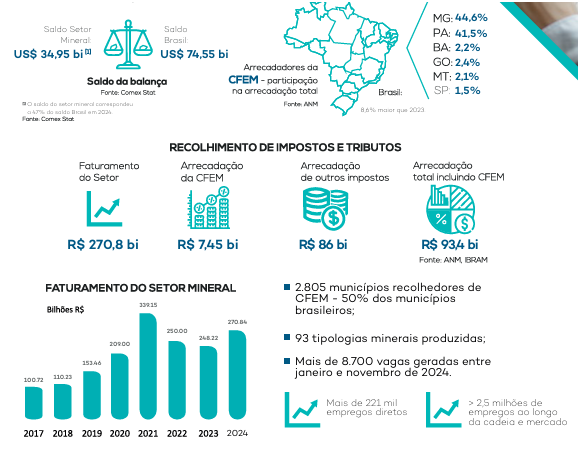
\includegraphics[width=\textwidth]{figures/image1_mineracao_numeros_1.png}
    \caption{Mineração em Números (2024) -- Saldo comercial, impostos e faturamento}
    \label{fig:image1_mineracao_numeros_1}
    \fonte{Mineração em Números (IBRAM, 2024)}
\end{figure}

\begin{figure}[!htb]
    \centering
    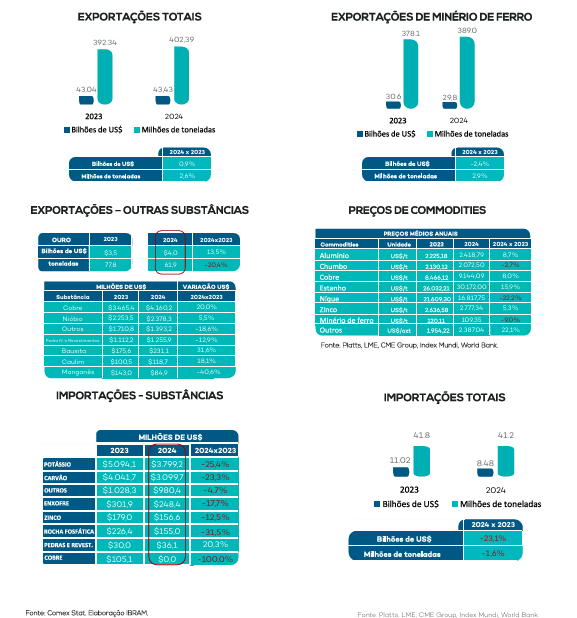
\includegraphics[width=\textwidth]{figures/image2_mineracao_numeros_2.png}
    \caption{Mineração em Números (2024) -- Exportação e Importação}
    \label{fig:image2_mineracao_numeros_2}
    \fonte{Mineração em Números (IBRAM, 2024)}
\end{figure}

\begin{figure}[!htb]
    \centering
    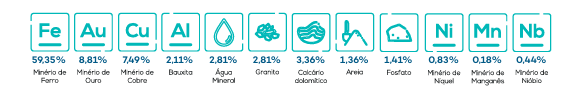
\includegraphics[width=\textwidth]{figures/image3_mineracao_numeros_3.png}
    \caption{Mineração em Números (2024) -- Principais substâncias produzidas -- Participação no faturamento do setor}
    \label{fig:image3_mineracao_numeros_3}
    \fonte{Mineração em Números (IBRAM, 2024)}
\end{figure}

\subsubsection{Geração de empregos}
\label{subsubsec:geracao_empregos}

Conforme a \citeauthor{anm2023informe3} (\citeyear{anm2023informe3}), para a análise do mercado de trabalho do Setor Mineral, são selecionados os grupos de atividades relevantes conforme a Classificação Nacional de Atividades Econômicas (CNAE) 2.0.

No estudo de \citeauthor{rocha2020impacto} (\citeyear{rocha2020impacto}), que visa avaliar o impacto macroeconômico da mineração no Brasil, é realizada uma distinção entre a Indústria Extrativa Mineral (IEM) e a Indústria de Transformação Mineral (ITM). Na Indústria Extrativa Mineral (IEM), refere-se à extração de minerais, incluem-se: extração de carvão mineral, extração de minério de ferro, extração de minerais metálicos não ferrosos, extração de pedra, areia e argila, extração de outros minerais não metálicos, e atividades de apoio à extração de minerais, exceto petróleo e gás natural. Na Indústria de Transformação Mineral (ITM), as atividades selecionadas são: fabricação de produtos cerâmicos, fabricação de artefatos de concreto, cimento, fibrocimento, gesso e materiais semelhantes, aparelhamento de pedras e fabricação de outros produtos de minerais não metálicos, siderurgia, fabricação de artigos de joalheria, bijuteria e semelhantes, produção de tubos de aço, exceto tubos sem costura, produção de ferro gusa e de ferroligas, fabricação de cimento, fabricação de produtos cerâmicos, e forjaria, estamparia, metalurgia do pó e serviços de tratamento de metais \cite{anm2023informe3}.

De acordo com \citeauthor{anm2023anuario} (\citeyear{anm2023anuario}), os detalhes sobre o Novo CAGED, e o CNAE 2.3, têm-se o seguinte, respectivamente:

\begin{quotation}
Até 2019, utilizou-se os dados do Cadastro Geral de Empregados e
Desempregados (CAGED), do Ministério da Economia (ME), formado por
trabalhadores celetistas. A partir de 2020, os dados passaram a ser
extraídos do Novo CAGED, que alterou a metodologia de coleta, conforme
Nota Técnica de 27/05/2020 do SEPRT/ME, ampliando a base avaliada para
todos os trabalhadores formais: empregados sob a CLT; temporários;
avulsos; agentes públicos; trabalhadores cedidos; dirigentes
sindicais; contribuintes individuais; e bolsistas.

Para a discriminação e totalização de dados de emprego específicos do
setor mineral dentro do Novo CAGED, o Informe seleciona os grupos de
atividades da Classificação Nacional das Atividades Econômicas (CNAE
2.3) a seguir: 50 - extração de carvão mineral; 71 - extração de
minério de ferro; 72 - extração de minerais metálicos não ferrosos;
81 - extração de pedra/areia/argila; 89 - extração de outros minerais
não metálicos e 99 - atividades de apoio à extração de minerais,
exceto petróleo e gás natural.
\end{quotation}

\paragraph{Indústria Extrativa Mineral (IEM)}

Segundo dados da \citeauthor{anm2023informe3} (\citeyear{anm2023informe3}), o saldo de emprego formal na Indústria Extrativa Mineral (IEM), calculado pela diferença entre admissões e demissões e fornecido pelo Novo CAGED (Cadastro Geral de Empregados e Desempregados no eSocial, fornecido pelo Ministério da Economia), registrou uma variação de 1.869 postos no terceiro trimestre de 2023; isso representa um aumento de 3,6\% em relação ao mesmo trimestre do ano anterior (03TRI2022), como pode ser observado na Figura \ref{fig:saldo_estoque_3tri2023}. Já no quarto trimestre, registrou variação de -119 vagas com carteira assinada; se comparado ao mesmo período do ano anterior, observa-se um aumento de 3,9\%; o setor mineral emprega diretamente 208.176 pessoas (Figura \ref{fig:saldo_estoque_4tri2023}).

\begin{figure}[!htb]
    \centering
    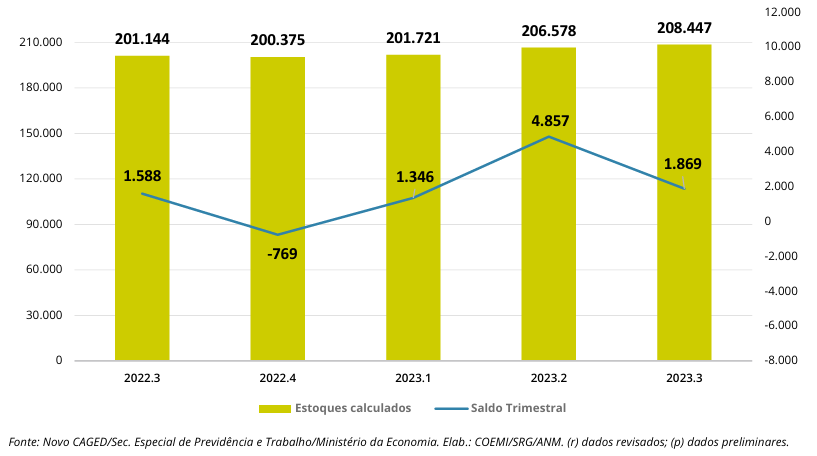
\includegraphics[width=\textwidth]{figures/image4_saldo_estoque_3tri2023.png}
    \caption{Saldo ajustado e estoque trimestral de mão de obra do setor de extração mineral (exceto petróleo e gás) -- 03TRI2023}
    \label{fig:saldo_estoque_3tri2023}
    \fonte{\citeauthor{anm2023informe3} (\citeyear{anm2023informe3})}
\end{figure}

\begin{figure}[!htb]
    \centering
    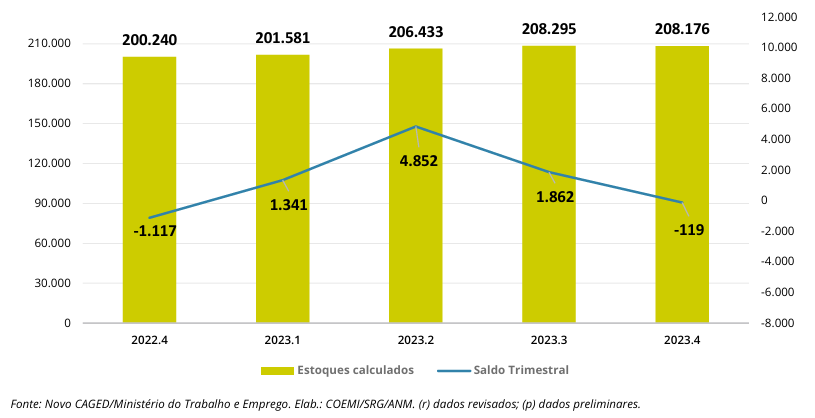
\includegraphics[width=\textwidth]{figures/image5_saldo_estoque_4tri2023.png}
    \caption{Saldo ajustado e estoque trimestral de mão de obra do setor de extração mineral (exceto petróleo e gás) -- 04TRI2023}
    \label{fig:saldo_estoque_4tri2023}
    \fonte{\citeauthor{anm2023informe4} (\citeyear{anm2023informe4})}
\end{figure}

Os resultados das contratações no Índice de Evolução do Mercado (IEM) demonstraram um saldo positivo durante o terceiro trimestre de 2023 para a maioria dos grupos classificados pelo Código Nacional de Atividades Econômicas (CNAE) 2.0, com exceção da atividade de Extração de Minerais Metálicos Não-Ferrosos (Figura \ref{fig:saldo_mao_obra_3tri2023}). A performance desfavorável neste grupo foi atribuída à interrupção das operações de extração de ouro pela AngloGold Ashanti, resultando no fechamento de 754 postos de trabalho em Santa Bárbara (MG). Além disso, contribuiu para esse resultado a falência da Buritirama Mineração, que atua na extração de manganês, ocasionando o encerramento de 408 postos de trabalho apenas em Marabá (PA) \cite{anm2023informe3}.

\begin{figure}[!htb]
    \centering
    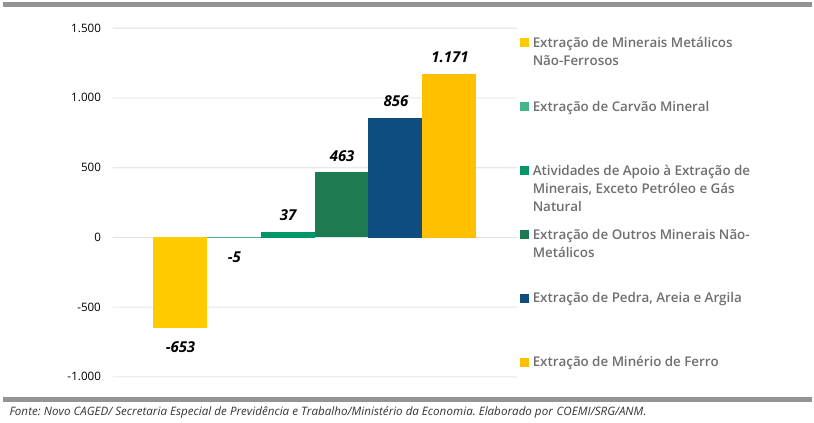
\includegraphics[width=\textwidth]{figures/image6_saldo_mao_obra_3tri2023.png}
    \caption{Saldo de mão de obra da indústria extrativa mineral (exceto petróleo e gás), por grupo CNAE 2.0 -- 03TRI2023}
    \label{fig:saldo_mao_obra_3tri2023}
    \fonte{\citeauthor{anm2023informe3} (\citeyear{anm2023informe3})}
\end{figure}

As flutuações anuais no número de trabalhadores contratados formalmente mostraram-se mais significativas no setor de Extração de Minério de Ferro (Figura \ref{fig:variacao_emprego_4tri2023}). Por outro lado, os resultados mais desfavoráveis foram observados no segmento das Atividades de Apoio à Extração de Minerais, com uma queda de 38,6\% \cite{anm2023informe4}.

\begin{figure}[!htb]
    \centering
    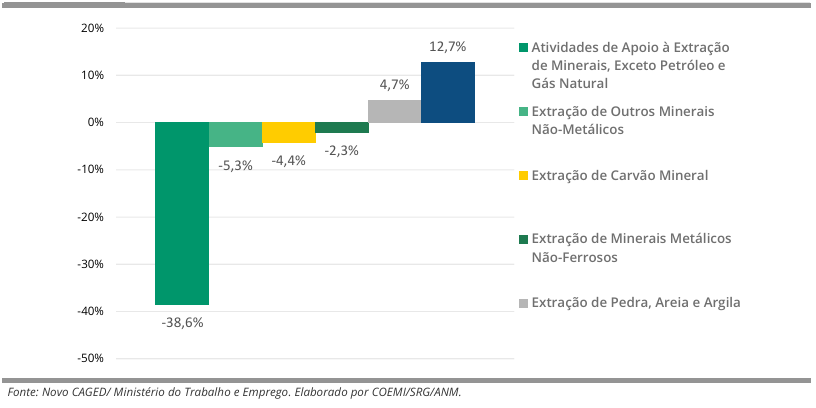
\includegraphics[width=\textwidth]{figures/image7_variacao_emprego_4tri2023.png}
    \caption{Variação interanual do emprego formal na indústria extrativa (exceto petróleo e gás), por grupo CNAE 2.0 -- 04TRI2023}
    \label{fig:variacao_emprego_4tri2023}
    \fonte{\citeauthor{anm2023informe4} (\citeyear{anm2023informe4})}
\end{figure}

A maior parte da distribuição da força de trabalho da IEM está concentrada nos estados de Minas Gerais (35\%), Pará (13\%), Bahia (7\%) e São Paulo (7\%), (Figura \ref{fig:estoque_mao_obra}) \cite{anm2023informe3}.

\begin{figure}[!htb]
    \centering
    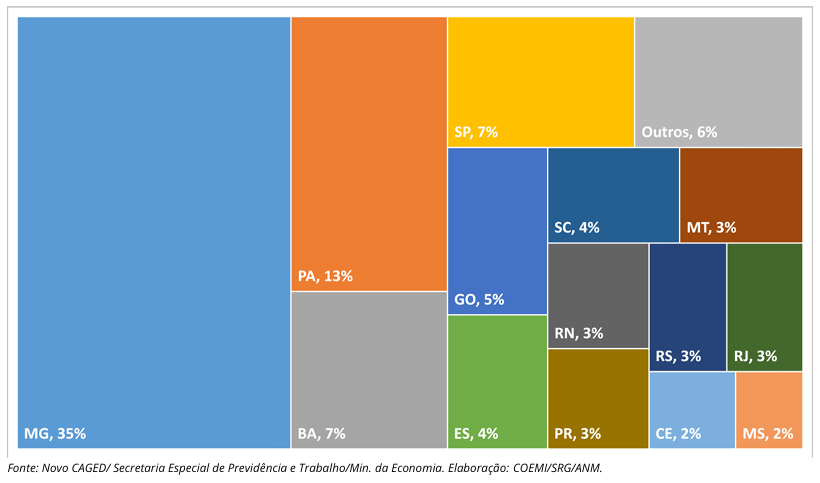
\includegraphics[width=\textwidth]{figures/image8_estoque_mao_obra.png}
    \caption{Estoque de mão de obra da IEM (exceto petróleo e gás) por estado}
    \label{fig:estoque_mao_obra}
    \fonte{\citeauthor{anm2023informe3} (\citeyear{anm2023informe3})}
\end{figure}

\paragraph{Indústria de Transformação Mineral (ITM)}

Pelos dados da \citeauthor{anm2023informe4} (\citeyear{anm2023informe4}), na Indústria de Transformação Mineral (ITM), os quatro principais setores empregadores são: Fabricação de Produtos Cerâmicos (18\%); Fabricação de Artefatos de Concreto, Cimento, Fibrocimento, Gesso e Materiais Semelhantes (17\%); Aparelhamento de pedras e fabricação de outros produtos de minerais não metálicos (12\%); Siderurgia (12\%); e Fundição (8\%) (Figura \ref{fig:distribuicao_itm}).

\begin{figure}[!htb]
    \centering
    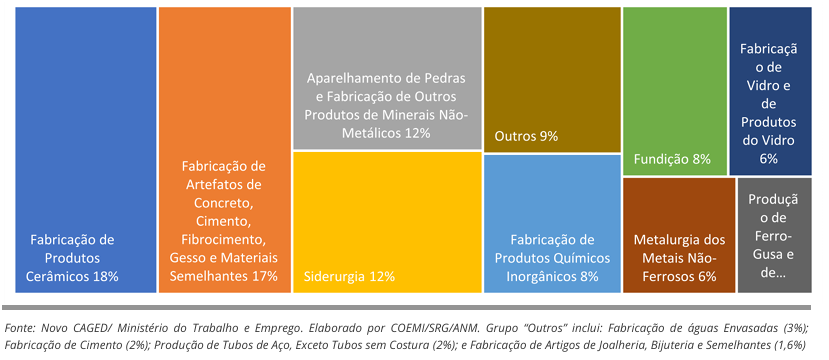
\includegraphics[width=\textwidth]{figures/image9_distribuicao_itm.png}
    \caption{Distribuição do estoque de mão de obra da ITM -- 04TRI2023}
    \label{fig:distribuicao_itm}
    \fonte{\citeauthor{anm2023informe4} (\citeyear{anm2023informe4})}
\end{figure}

No quarto trimestre de 2023, os níveis de emprego na ITM atingiram 718.631 postos, representando uma leve redução de 0,3\% em comparação com o quarto trimestre de 2022 (Figura \ref{fig:evolucao_saldo_itm}). Na Figura \ref{fig:salarios_admissao}, a mediana dos salários de admissão no setor de Indústria Extrativa Mineral foi de R\$ 1.988,67.

\begin{figure}[!htb]
    \centering
    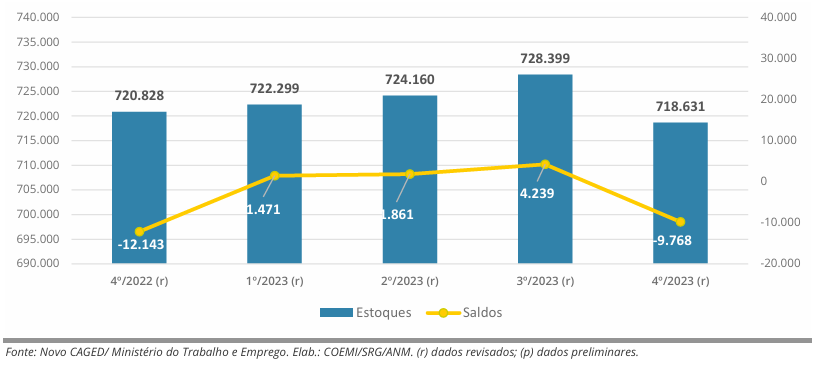
\includegraphics[width=\textwidth]{figures/image10_evolucao_saldo_itm.png}
    \caption{Evolução do saldo e do estoque de trabalhadores da ITM -- 04TRI2022 a 04TRI2024}
    \label{fig:evolucao_saldo_itm}
    \fonte{\citeauthor{anm2023informe4} (\citeyear{anm2023informe4})}
\end{figure}

\begin{figure}[!htb]
    \centering
    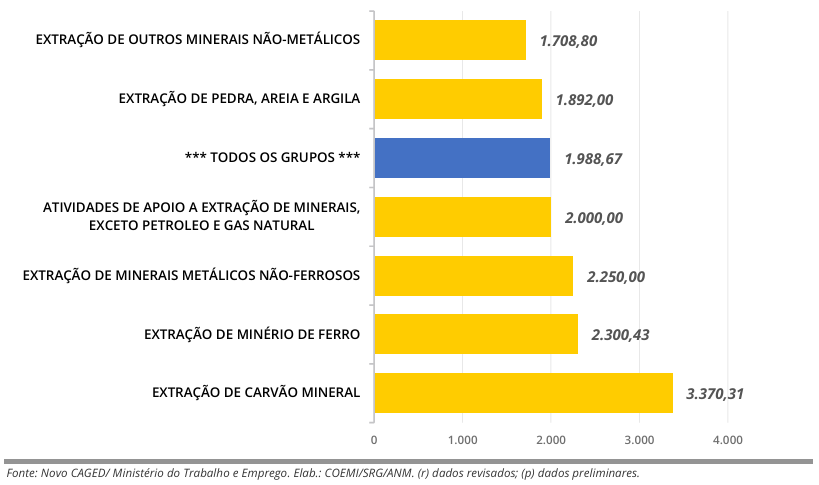
\includegraphics[width=\textwidth]{figures/image11_salarios_admissao.png}
    \caption{Salários de admissão na extração mineral na IEM -- 04TRI2023}
    \label{fig:salarios_admissao}
    \fonte{\citeauthor{anm2023informe4} (\citeyear{anm2023informe4})}
\end{figure}

\subsection{Geração de resíduos (sólidos, líquidos, gasosos)}
\label{subsec:geracao_residuos}

Nessa sessão apresenta-se uma visão da geração de resíduos minerais.

Os bens minerais são divididos em duas grandes categorias: os minerais não metálicos e os metálicos. De acordo com os dados do Anuário Mineral Brasileiro \cite{anm2022anuario}, os minerais metálicos responderam por 89\% do valor da produção mineral brasileira em 2021, como pode ser observado na Figura \ref{fig:participacao_minerais}. Dentre as substâncias, onze evidenciam-se por corresponderem a
99,7\% do valor da produção da referida classe, quais sejam: alumínio, cobre, cromo, estanho, ferro, manganês, nióbio, níquel, ouro, vanádio e zinco. O mineral de ferro concentra 80,1\% desse volume. O valor da produção dessas onze substâncias totalizou 312,9 bilhões de reais, com destaque para a expressiva participação do ferro nesse montante, cuja produção é concentrada, principalmente, nos estados do Pará e Minas Gerais.

\begin{figure}[!htb]
    \centering
    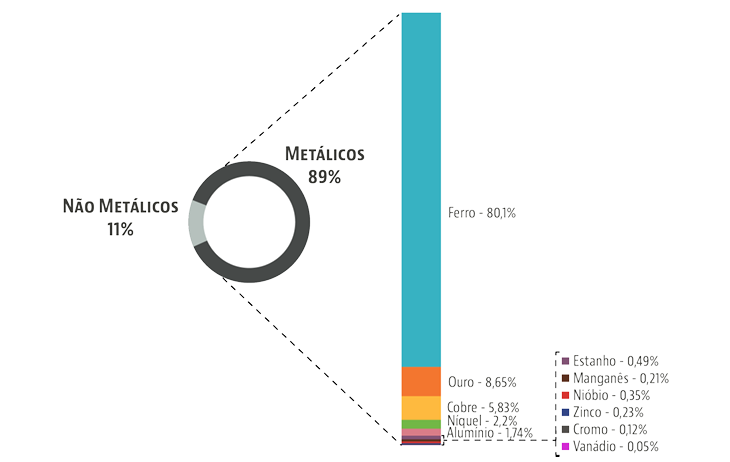
\includegraphics[width=0.93\textwidth]{figures/image12_participacao_minerais.png}
    \caption{Participação das principais substâncias metálicas no valor da produção mineral comercializada - 2021}
    \label{fig:participacao_minerais}
    \fonte{\citeauthor{anm2022anuario} (\citeyear{anm2022anuario})}
\end{figure}

Os bens minerais não metálicos, que compuseram 11\% do valor da produção mineral em 2021, podem ser categorizados, em 7 categorias, da seguinte forma \cite{carvalho2018sustentabilidade}:

\begin{enumerate}
    \item Rochas e Minerais Industriais: Inclui materiais como grafita, magnesita, crisotila, calcário, areia industrial, barita, bentonita e fluorita, utilizados principalmente em aplicações industriais;
    
    \item Rochas Ornamentais e de Revestimento: Engloba granitos, mármores, ardósias e quartzitos, valorizados por suas propriedades estéticas e de revestimento;
    
    \item Materiais para Construção Civil: Compreende areia, brita e argila, essenciais na construção de infraestruturas civis;
    
    \item Agrominerais: Inclui rochas fosfáticas e calcário agrícola, utilizados na agricultura para melhorar a qualidade do solo;
    
    \item Minerais Energéticos: Como o carvão mineral, utilizado como fonte de energia;
    
    \item Pedras Preciosas e Semipreciosas: Inclui gemas como diamantes, rubis, esmeraldas, entre outros; e
    
    \item Água Mineral: Água proveniente de fontes naturais com propriedades físicas e químicas distintas, utilizada para consumo humano.
\end{enumerate}

Os minerais metálicos são classificados em três categorias principais \cite{carvalho2018sustentabilidade}:

\begin{enumerate}
    \item metais ferrosos, que incluem elementos como ferro, nióbio, manganês e cromo;
    
    \item metais não ferrosos, abrangendo alumínio, cobalto, cobre, chumbo, estanho, metais do grupo da platina, tálio, tântalo, terras-raras, titânio, vanádio, molibdênio e zinco; e
    
    \item metais preciosos, como ouro e prata.
\end{enumerate}

A produção dos principais minerais metálicos no Brasil está apresentada na Tabela \ref{tab:producao-minerais}.

\begin{table}[!htb]
    \centering
    \ABNTEXfontereduzida
    \captionsetup{justification=centering}
    \caption{Produção dos principais minerais metálicos no Brasil, em 2021}
    \label{tab:producao-minerais}
    \begin{tabular}{|p{4cm}|p{3cm}|p{3cm}|p{3cm}|}
        \hline
        \textbf{Substância mineral} & \textbf{Quantidade bruta (ROM) (t)} & \textbf{Quantidade beneficiada (t)} & \textbf{Valor total (R\$)} \\
        \hline
        Ferro & 567.770.006 & 430.550.725 & 250.698.910.257 \\
        Ouro & 77.711.602 & 62.215 (kg) & 18.334.390.096 \\
        Cobre & 99.573.449 & 1.152.696 & 18.249.632.321 \\
        Níquel & 12.448.552 & 342.268 & 6.896.739.348 \\
        Alumínio (bauxita) & 46.319.730 & 33.364.875 & 5.436.681.849 \\
        Estanho (cassiterita) & 24.147.707 & 27.234.898 (kg) & 1.544.151.737 \\
        Nióbio & 23.032.412 & 209.300 & 1.098.461.500 \\
        Manganês & 1.775.218 & 1.426.058 & 625.957.307 \\
        \hline
    \end{tabular}
    \fonte{\citeauthor{anm2022anuario} (\citeyear{anm2022anuario})}
\end{table}

O mineral metálico de maior volume de produção é o minério de ferro. Entre os minerais não metálicos, os agregados para construção civil, como brita, cascalho, areia e calcário são consumidos quase em seu estado bruto, já a produção de minério de ferro requer processos de concentração. Esses processos fazem com que o minério de ferro gere o maior volume de rejeitos minerais no país \cite{carvalho2018sustentabilidade}.

O minério de ferro é responsável pela maioria das grandes minas no Brasil, com 46 das 76 grandes minas mapeadas em 2021, conforme indicado na Figura \ref{fig:porte_lavra}.

\begin{figure}[!htb]
    \centering
    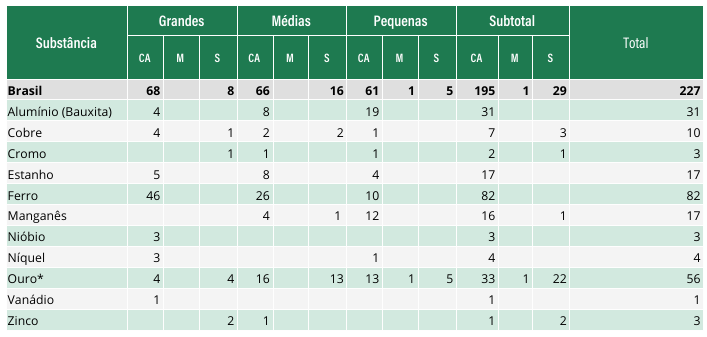
\includegraphics[width=0.8\textwidth]{figures/image13_porte_lavra.png}
    \caption{Porte e modalidade de lavra das minas - 2021}
    \label{fig:porte_lavra}
    \fonte{\citeauthor{anm2022anuario} (\citeyear{anm2022anuario})}
\end{figure}

\textbf{Nota:} Grande: produção bruta (ROM) anual maior que 1.000.000 t; Média: maior que 100.000 t até 1.000.000 t; Pequena: maior que 10.000 t até 100.000 t; CA: mina a céu aberto; M: mina mista (subterrânea e céu aberto); S: mina subterrânea.

Com um número elevado de jazidas e alta produção de minerais metálicos no Brasil, o minério de ferro representa o principal componente mineral da balança de exportação do país, totalizando US\$ FOB 44,6 bilhões em 2021. Mais de 90\% da utilização desse recurso é direcionada à fabricação
de aço \cite{carvalho2014minerio}. No contexto da produção global de minério de ferro, o Brasil ocupa a posição de segundo maior fornecedor do mundo, sendo superado apenas pela Austrália. Os dados da produção de 2020 e 2021, assim como informações sobre reservas lavráveis e teor de ferro dos principais produtores globais, estão detalhados na Tabela \ref{tab:producao-reservas} da U.S. Geological Survey \cite{usgs2022iron}.

\begin{table}[!htb]
    \centering
    \caption{Produção e reservas mundiais de minério de ferro (milhões de t), em 2020 e 2021}
    \label{tab:producao-reservas}
    \resizebox{\textwidth}{!}{%
    \begin{tabular}{lccccccc}
        \hline
        & \multicolumn{4}{c}{\textbf{Produção mineral (milhões de t)}} & \multicolumn{3}{c}{\textbf{Reservas (milhões de t)}} \\
        \cline{2-5} \cline{6-8}
        & \multicolumn{2}{c}{Minério} & \multicolumn{2}{c}{Conteúdo de ferro} & Minério & Conteúdo & Fe \\
        & 2020 & 2021 & 2020 & 2021 & bruto & de ferro & (\%) \\
        \hline
        Austrália & 912,000 & 900,000 & 565,000 & 560,000 & 51,000 & 25,000 & 33 \\
        Brasil & 388,000 & 380,000 & 247,000 & 240,000 & 34,000 & 15,000 & 44 \\
        China & 360,000 & 360,000 & 225,000 & 220,000 & 20,000 & 6,900 & 35 \\
        Índia & 204,000 & 240,000 & 127,000 & 150,000 & 5,500 & 3,400 & 62 \\
        Rússia & 100,000 & 100,000 & 69,500 & 71,000 & 25,000 & 14,000 & 56 \\
        Ucrânia & 78,800 & 81,000 & 49,300 & 51,000 & 6,500 & 2,300 & 35 \\
        Canadá & 60,100 & 68,000 & 36,100 & 41,000 & 6,000 & 2,300 & 38 \\
        Cazaquistão & 62,900 & 64,000 & 12,700 & 13,000 & 2,500 & 900 & 36 \\
        África do Sul & 55,600 & 61,000 & 35,400 & 39,000 & 1,000 & 670 & 67 \\
        Irã & 49,500 & 50,000 & 32,500 & 33,000 & 2,700 & 1,500 & 55 \\
        EUA & 38,100 & 46,000 & 24,100 & 29,000 & 3,000 & 1,000 & 33 \\
        Suécia & 35,800 & 40,000 & 25,400 & 28,000 & 1,300 & 600 & 46 \\
        Chile & 15,600 & 19,000 & 9,890 & 12,000 & N/A & N/A & N/A \\
        Turquia & 15,400 & 16,000 & 8,570 & 8,900 & 130 & 38 & 29 \\
        México & 14,900 & 17,000 & 9,380 & 11,000 & N/A & N/A & N/A \\
        Peru & 13,300 & 16,000 & 8,890 & 11,000 & 2,600 & 1,500 & 58 \\
        Outros países & 69,500 & 90,000 & 40,000 & 58,000 & 18,000 & 9,500 & 53 \\
        \hline
        Total mundo & 2,470,000 & 2,600,000 & 1,520,000 & 1,600,000 & 180,000 & 85,000 & 47 \\
        \hline
    \end{tabular}%
    }
    \fonte{\citeauthor{usgs2022iron} (\citeyear{usgs2022iron})}
\end{table}

Segundo \cite{usgs2024iron}, produção de minério de ferro, em milhões de t, nos
anos 2022 e 2023, foram de respectivamente, 435.000 e 440.000.

A tendência é que a mineração continue crescendo tanto em termos de
produção quanto de importância econômica. Consequentemente, os impactos
socioambientais também aumentam. Entre os principais riscos para as
populações e regiões afetadas estão o tamanho das operações minerais, o
volume de carga movimentada e a quantidade de resíduos gerados. Esses
riscos são exacerbados por acidentes e pela ineficiência nos mecanismos
de deposição e monitoramento dos rejeitos, especialmente no caso do
minério de ferro, em que o Brasil se destaca mundialmente em produção
\cite{carvalho2018sustentabilidade}.

A atividade de mineração compreende um conjunto de processos técnicos e
operacionais, conforme estabelecido pelo Decreto nº 9.406/2018, Art. 5º,
que incluem pesquisa geológica, desenvolvimento da mina, lavra,
beneficiamento dos minérios, transporte, comercialização, gestão
(aproveitamento) de resíduos, o armazenamento de estéreis e rejeitos e o
fechamento da mina \cite{decreto9406_2018}.

O setor de mineração pode ser compreendido nas seguintes etapas, como
também pode ser observado na Figura \ref{fig:etapas_mineracao}. As três primeiras etapas visam ao
mapeamento e ao processamento dos recursos minerais. Os recursos
minerais são depósitos de minério cujas propriedades permitem a extração
de maneira técnica e economicamente viável para a produção de bens
minerais. A etapa final da mineração envolve a recuperação ambiental das
áreas afetadas. \cite[p.340-341]{carvalho2018sustentabilidade}:

\begin{enumerate}
    \item Prospecção: Fase inicial que envolve a busca e identificação
    preliminar de depósitos minerais em uma determinada área geográfica;

    \item Pesquisa Mineral: Consiste na realização de estudos detalhados e
    análises geológicas para confirmar a presença e a viabilidade
    econômica dos depósitos minerais identificados durante a prospecção;

    \item Lavra: Processo de extração dos minerais do solo, que pode incluir
    métodos de mineração a céu aberto ou subterrânea, além do
    beneficiamento dos minérios extraídos; e

    \item Descomissionamento de Mina: Etapa final que envolve o fechamento e
    reabilitação da mina, garantindo que a área seja estabilizada e
    restaurada de acordo com normas ambientais e de segurança, visando
    minimizar impactos ambientais a longo prazo.
\end{enumerate}

\begin{figure}[!htb]
    \centering
    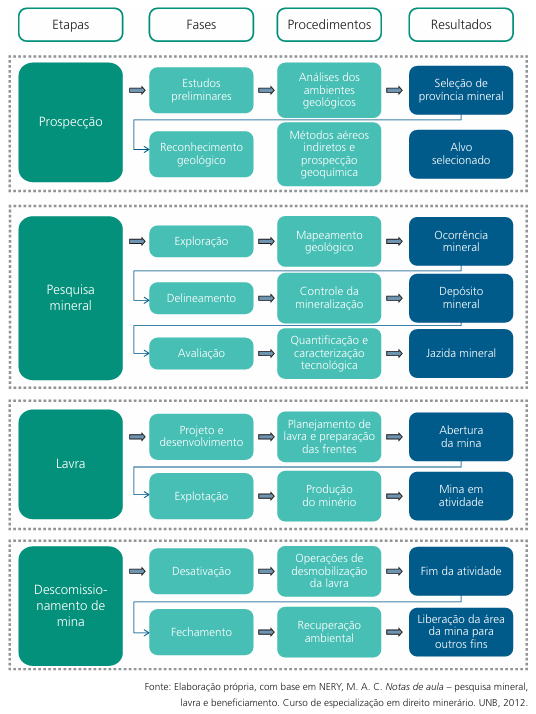
\includegraphics[width=0.9\textwidth]{figures/image14_etapas_mineracao.png}
    \caption{Etapas da mineração.}
    \label{fig:etapas_mineracao}
    \fonte{\citeauthor{carvalho2018sustentabilidade} (\citeyear{carvalho2018sustentabilidade})}
\end{figure}

As etapas e os procedimentos de mineração englobam um conjunto de
processos essenciais para a obtenção de um produto mineral bruto, um
concentrado ou aglomerado. O beneficiamento mineral, que constitui a
fase final da lavra e inclui a aglomeração, envolve exclusivamente
alterações físicas no minério.

A seguir, são descritos os processos e as atividades associadas a cada
etapa, com ênfase particular nas fases de lavra e descomissionamento de
mina, devido ao seu significativo impacto nos ambientes mineiros \cite[p.342]{carvalho2018sustentabilidade}.

A fase de prospecção, segundo \cite[p.342]{carvalho2018sustentabilidade},
``subdividida em estudos preliminares e no reconhecimento geológico,
engloba procedimentos como análises dos ambientes geológicos, métodos
aéreos indiretos e prospecção geoquímica. Os resultados obtidos nessa
etapa são a seleção de província mineral e do alvo a pesquisar.''.

A pesquisa geológica divide em exploração, delineamento e avaliação,
utilizando técnicas como mapeamento geológico, análise da mineralização,
quantificação e caracterização tecnológica. Durante este estágio, são
detalhadas a presença do mineral, a extensão do depósito e a natureza da
jazida, avaliando-se a viabilidade de sua exploração econômica \cite{carvalho2018sustentabilidade}.

No Brasil, o Decreto-lei nº 227, de 28 de fevereiro de 1967 (Código de
Mineração), em seu Capítulo III, Artigo 36, determina que, a lavra é o
conjunto coordenado de operações destinadas ao aproveitamento industrial
da jazida, compreendendo desde a extração dos minerais até seu
beneficiamento. Durante esta fase, destacam-se atividades como projeto e
desenvolvimento da mina, preparação das frentes de lavra, abertura da
mina, extração do minério e beneficiamento, sendo a etapa mais intensiva
na geração de resíduos (sólidos, líquidos e gasosos) \cite{brasil1967decreto}.

Por envolver atividades com alto impacto ambiental, o início da etapa de
lavra depende, em geral, de estudo de impacto ambiental (EIA), e seu
respectivo relatório de impacto ambiental (Rima), e da licença ambiental
dos órgãos competentes \cite[p.342]{carvalho2018sustentabilidade}.

Ainda segundo \cite[p.343]{carvalho2018sustentabilidade}, a seleção do método de
lavra é um fator crucial que viabiliza a operação de extração do
material mineral. As propriedades físicas do depósito, tais como
profundidade, extensão e inclinação do corpo mineralizado, impõem
restrições à aplicação de determinados métodos de lavra.

Além desses fatores, outras questões devem ser avaliadas, incluindo as
técnicas de drenagem e bombeamento das águas superficiais e
subterrâneas, a permeabilidade, a deformabilidade e a resistência da
rocha \cite[p.343]{carvalho2018sustentabilidade}.

De acordo com \cite{minasjr2019lavra}, esse processo é classificado em dois
grandes grupos: lavra subterrânea e superficial (a céu aberto). Esta
classificação baseia-se nas distintas técnicas de extração do minério,
denominadas métodos de lavra, utilizadas em cada grupo.

O método de lavra a céu aberto refere-se à extração de materiais por
meio de escavações realizadas diretamente na superfície terrestre. Em
geral, a espessura do estéril --- material sem valor econômico que
recobre o minério --- é relativamente pequena, ou a estrutura geológica
do depósito torna inviável ou economicamente desfavorável a abertura de
túneis. O acesso ao minério nessas minas é realizado através do processo
de decapeamento, que envolve a remoção e o transporte da camada
superficial do solo. Subsequentemente, procede-se à remoção do solo
alterado. Os principais minerais extraídos por métodos de lavra a céu
aberto incluem talco, quartzo, argilas, esmeralda, diamante, brita,
ouro, areia e cascalho.

Já o método de lavra subterrânea ocorre no interior do terreno, sendo
adequada para rochas e minerais situados em depósitos mais profundos.
Nesses casos, a relação estéril-minério é alta, tornando economicamente
inviável a exploração a céu aberto. Além disso, há situações em que a
legislação exige a lavra subterrânea.

O acesso ao minério em minas subterrâneas é geralmente feito através de
poços verticais perfurados a partir da superfície, conhecidos como
shafts. Esses shafts permitem o trânsito de pessoas, equipamentos,
suprimentos e o próprio minério. A partir dos shafts, são escavadas
galerias horizontais, chamadas de drifts, para a extração do minério.

Além dos shafts e drifts, existem rampas, que são galerias de baixa
inclinação e curvilíneas destinadas ao tráfego de veículos. Os slopes
são galerias de baixa inclinação usadas para o transporte de correias
transportadoras. As chaminés, aberturas verticais, são utilizadas para a
passagem de material, ventilação e servem como rotas de fuga, embora
normalmente não alcancem a superfície.

A Figura \ref{fig:metodos_lavra} apresenta uma descrição detalhada dos métodos de lavra
\cite{freire2020rejeitos}.

\begin{figure}[!htb]
    \centering
    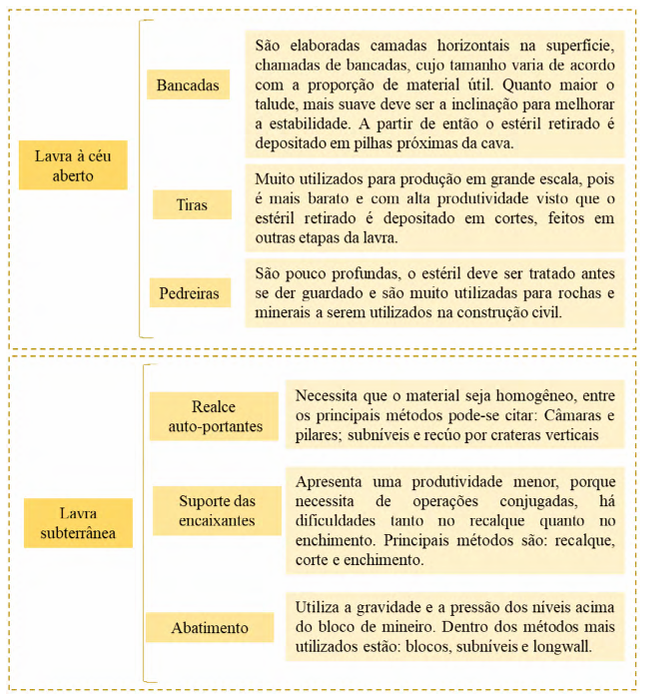
\includegraphics[width=0.9\textwidth]{figures/image15_metodos_lavra.png}
    \caption{Métodos de Lavra.}
    \label{fig:metodos_lavra}
    \fonte{\citeauthor{minasjr2019lavra} (\citeyear{minasjr2019lavra}) apud \citeauthor{freire2020rejeitos} (\citeyear{freire2020rejeitos})}
\end{figure}

Quando comparadas entre si, as operações de lavra a céu aberto
apresentam diversas vantagens, incluindo menor custo de produção,
facilidade de supervisão, melhores condições de trabalho, uso mais
racional e eficiente de explosivos, menores riscos, maior nível de
produção e utilização de equipamentos de grande porte. No entanto, as
desvantagens desse método incluem a necessidade de maior movimentação de
materiais, a imobilização de grandes áreas, a exposição dos
trabalhadores às intempéries e a limitação da profundidade de extração
\cite{freire2020rejeitos}.

No Brasil, a maior parte das operações de mineração no Brasil é
realizada em minas a céu aberto \cite[p.343]{carvalho2018sustentabilidade}.

\cite{carvalho2018sustentabilidade} destacam que a etapa de lavra é a fase de maior
intensidade na geração de efluentes (sólidos, líquidos e gasosos). Esta
etapa abrange as seguintes atividades: projeto e desenvolvimento da
mina, preparação das frentes de lavra, abertura da mina, extração do
minério e beneficiamento. As operações de lavra são ilustradas na Figura \ref{fig:operacoes_lavra}.

\begin{figure}[!htb]
    \centering
    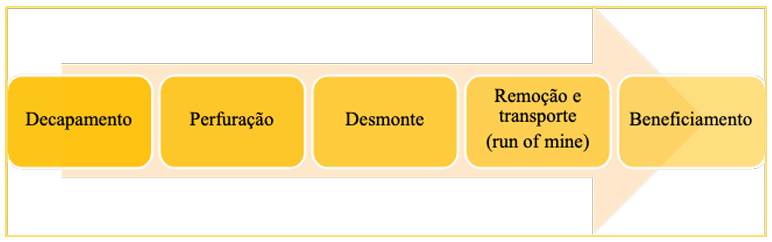
\includegraphics[width=0.9\textwidth]{figures/image16_operacoes_lavra.png}
    \caption{Operações de lavra.}
    \label{fig:operacoes_lavra}
    \fonte{\citeauthor{carvalho2018sustentabilidade} (\citeyear{carvalho2018sustentabilidade}), p. 344 apud \citeauthor{freire2020rejeitos} (\citeyear{freire2020rejeitos})}
\end{figure}

A remoção de material superficial é realizada durante a abertura e
desenvolvimento da mina, processo conhecido como decapeamento, visando
expor a rocha de interesse, denominada estéril. Na fase de perfuração,
utilizam-se máquinas hidráulicas que executam furos com diâmetro,
comprimento e distâncias previamente calculados. Desvios na perfuração
podem resultar em problemas e danos estruturais durante a fase de
desmonte. O desmonte pode ser realizado de maneira mecânica ou através
da combinação de perfuração e detonação. O minério fragmentado, com
valor econômico, conhecido como run of mine, é transportado para a
unidade de beneficiamento. Nesta unidade, são realizados processos que
têm como objetivo promover a separação física do run of mine da ganga,
ou seja, da parte sem interesse econômico ou rejeitada, para obter um
concentrado com maior teor de concentração mineral \cite[p.345-346]{carvalho2018sustentabilidade}. Nessa fase, ocorre a produção de uma quantidade
significativa de resíduos, que quando misturados à água, são denominados
rejeitos \cite[apud][]{freire2020rejeitos}.

Finalmente, a fase derradeira da atividade de mineração compreende o
encerramento da operação da mina, envolvendo o descomissionamento que
abrange procedimentos essenciais para sua inativação: desmobilização,
encerramento e reabilitação ambiental, visando a devolução do local para
outros usos pela comunidade. É crucial manter o monitoramento dos
efeitos residuais, mesmo após a restauração completa da área \cite{carvalho2018sustentabilidade}.

\subsubsection{Gestão de resíduos sólidos e métodos de disposição de rejeitos}
\label{subsubsec:gestao_residuos}

Na atividade mineradora, os principais fatores de riscos e impactos
ambientais derivam da presença de: (i) materiais sólidos removidos
durante a extração, conforme já mencionado, na fase 1 da lavra, no
decapeamento, geralmente permanecendo na área de mineração, os resíduos
sólidos de extração, conhecidos como estéril; e (ii) resíduos do
tratamento/beneficiamento, denominados rejeitos. A gestão desses
materiais envolve o planejamento e a disposição adequada dos resíduos
gerados, incluindo sua recuperação ou reutilização, além da
monitorização das estruturas de armazenamento e dos materiais
depositados \cite[p.357]{carvalho2018sustentabilidade}.

A Figura \ref{fig:producao_minerio} quantifica a quantidade de material estéril e rejeitos
proveniente da extração de minério de ferro no Brasil, utilizando
informações dos relatórios anuais de operação submetidos ao Departamento
Nacional de Produção Mineral (DNPM) e projeções de produção futura
\cite[p.358]{carvalho2018sustentabilidade}.

\begin{figure}[!htb]
    \centering
    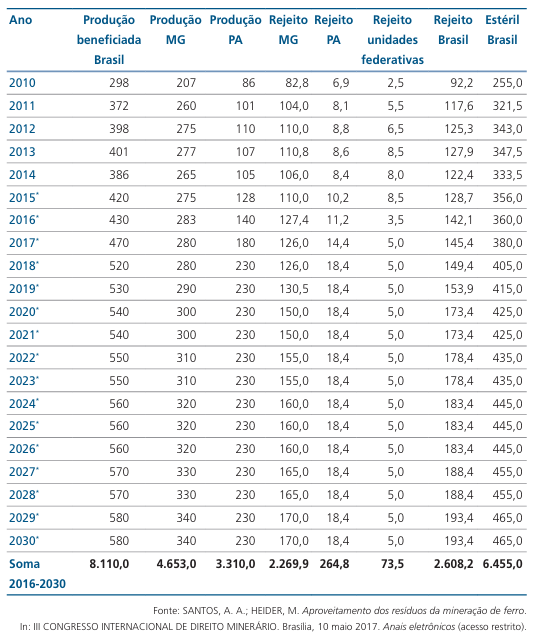
\includegraphics[width=0.9\textwidth]{figures/image17_producao_minerio.png}
    \caption{Produção beneficiada de minério de ferro, volume de rejeito e de estéril (milhões de t).}
    \label{fig:producao_minerio}
    \fonte{\citeauthor{carvalho2018sustentabilidade} (\citeyear{carvalho2018sustentabilidade})}
\end{figure}

\subsubsection{Resíduos sólidos de extração -- estéril}
\label{subsubsec:esteril}

Materiais estéreis são substâncias inertes resultantes do decapeamento
superficial durante a mineração, geralmente mantidas na própria mina em
pilhas ou utilizadas para o preenchimento de cavas exauridas. O volume
de estéril gerado é influenciado pelas características geológicas da
região de mineração e é determinado pela razão de estéril, que
representa a relação entre a quantidade de estéril a ser removida e a
quantidade de minério bruto lavrado \cite[p.359]{carvalho2018sustentabilidade};
essa produção bruta de minério, frequentemente referida como Run-of-Mine
(ROM), representa a quantidade total de minério extraído diretamente da
mina em um determinado ano, sem passar por qualquer processo de
beneficiamento ou tratamento \cite{anm2022anuario}.

\subsubsection{Resíduos sólidos de beneficiamento -- rejeito}
\label{subsubsec:rejeitos}

O rejeito é a fração descartada do minério bruto durante o processo de
beneficiamento para a obtenção do concentrado, utilizando métodos
mecânicos e/ou químicos. Este material é considerado não economicamente
viável para aproveitamento sob as condições atuais no momento de sua
geração.

As características dos rejeitos variam conforme o tipo de mineral e seu
tratamento na planta de beneficiamento. Os rejeitos podem ser finos,
compostos por siltes. Silte refere-se a partículas de minerais ou rochas
menores que areia finas e maiores que argila, com diâmetro entre 4 µm e
64 µm, de acordo com a escala de Wentworth amplamente utilizada em
geologia. Segundo a Associação Brasileira de Normas Técnicas (ABNT), NBR
6502, que trata de rochas e solos, define-se silte como solo com baixa
ou nenhuma plasticidade e que exibe baixa resistência quando seco ao ar.
As propriedades dominantes de um solo específico são devidas à fração de
silte. Estes rejeitos finos podem ser depositados na forma de lama
(polpa). Alternativamente, os rejeitos podem ser formados por materiais
arenosos, com granulometria mais grossa, conhecidos como rejeitos
granulares.

Os rejeitos granulares apresentam elevada permeabilidade, resistência
significativa ao cisalhamento e eficiente capacidade de sedimentação,
propriedades que favorecem sua estabilização em depósitos. Em contraste,
os rejeitos de granulometria fina, conhecidos como lamas, apresentam
desafios consideráveis no processo de sedimentação.

Durante o processo de deposição de resíduos, o intervalo de tempo entre
a aplicação de camadas sucessivas é ajustado para permitir a secagem
adequada da camada anterior, promovendo assim um aumento na resistência
do material depositado. Uma velocidade de deposição excessivamente alta
pode comprometer essa secagem, resultando em ressecamento parcial e
potencialmente facilitando a liquefação do resíduo. Isso pode reduzir a
resistência ao cisalhamento e aumentar a suscetibilidade a rupturas no
depósito \cite[p.360-361]{carvalho2018sustentabilidade}.

\subsubsection{Métodos de disposição de rejeitos}
\label{subsubsec:metodos_disposicao}

A escolha do método de disposição de rejeitos é determinada pela
natureza do processo de mineração, pelas condições geológicas e
topográficas locais, pelas propriedades mecânicas dos materiais, pelo
potencial de impacto ambiental dos contaminantes presentes nos rejeitos,
e pelas condições climáticas da região \cite{ibram2016gestao}.

Há três formas de disposição de rejeito: os métodos a céu aberto,
subterrâneos ou subaquáticos. A disposição a céu aberto é frequentemente
realizada através de pilhas controladas ou estruturas de contenção em
bacias ou vales. A disposição subterrânea ocorre por meio de câmaras
abertas após a extração do minério, onde os rejeitos são bombeados para
preenchê-las. A disposição subaquática, pouco utilizada devido aos
impactos negativos significativos nos ecossistemas, pode resultar em
impactos irreversíveis \cite{erazo2006selecao}.

Normalmente, os rejeitos são depositados em minas subterrâneas, cavas
esgotadas de mineração, pilhas através do método de empilhamento a seco
(dry stacking), deposição em forma de pasta, e barragens de contenção de
rejeitos \cite{ibram2016gestao}.

A disposição de resíduos em reservatórios formados por estruturas de
contenção como diques ou barragens é o método predominante. As barragens
constituem-se como mais utilizados para a disposição de rejeitos por
meio do aterro hidráulico, em virtude da possibilidade de conter um
grande volume de material com custos menores (THOMÉ; LAGO, 2017). Essas
estruturas podem ser compostas por solo natural ou construídas
utilizando os próprios resíduos, sendo categorizadas, respectivamente,
como barragens de contenção alteadas com resíduos e barragens
convencionais de solo natural. Muitos resíduos são transportados para a
área de disposição com uma alta umidade, variando de 10\% a 25\% de
sólidos \cite{ibram2016gestao}.

De acordo com a NBR 13028/2017, as barragens são definidas como:

\begin{citacao}
Barragens, barramentos, diques, reservatórios, cavas exauridas com
barramentos construídos, associados às atividades desenvolvidas com
base em direito minerário, utilizados para fins de contenção,
acumulação ou decantação de rejeito de mineração ou descarga de
sedimentos provenientes de atividades em mineração, com ou sem
captação de água associada, compreendendo a estrutura do barramento e
suas estruturas associadas. \cite[3.4]{abnt2017nbr13028}
\end{citacao}

Ao contrário das represas convencionais, destinadas à retenção de água,
as barragens de rejeitos são estruturas projetadas para armazenar
materiais resultantes de processos de beneficiamento mineral, os quais
possuem composições iônicas distintas. Essas composições são
potencialmente prejudiciais tanto para a saúde humana quanto para o meio
ambiente, além de poderem afetar negativamente a integridade da
estrutura ao interagirem com os materiais utilizados na construção do
aterro, provocando alterações em sua permeabilidade \cite{cardozo2017metodos}.

Além disso, o barramento não é construído de forma contínua, como é
típico em projetos convencionais; o aumento da altura do dique inicial
ocorre progressivamente conforme o avanço da mineração, utilizando
materiais provenientes de áreas de empréstimo ou do próprio rejeito. Os
métodos predominantes para o aumento construtivo da altura são:
montante, jusante ou ao longo da linha de centro, os quais serão
descritos em detalhes no próximo segmento \cite[p.12]{ibram2016gestao}.

A seleção entre métodos de execução é determinada por uma variedade de
variáveis técnicas e econômicas, incluindo o tipo de processo
industrial, características geotécnicas, volume de produção de rejeitos,
demandas de reservação e controle de água percolada, sismicidade,
topografia, hidrologia, hidrogeologia e custos associados. As barragens
alteadas pelo método de montante emergem como preferenciais entre as
empresas mineradoras devido à sua facilitação de execução e maior
viabilidade econômica \cite[p.17]{ibram2016gestao}.

\subsection{Tipos de barragens de rejeitos}
\label{subsec:tipos_barragens}

Barragens de rejeitos são reservatórios feitos com o objetivo de reter
água e resíduos sólidos resultantes da extração de minérios para que
evite danos ambientais. (OBTER O TEXTO FINAL - RENATA)

\begin{figure}[!htb]
    \centering
    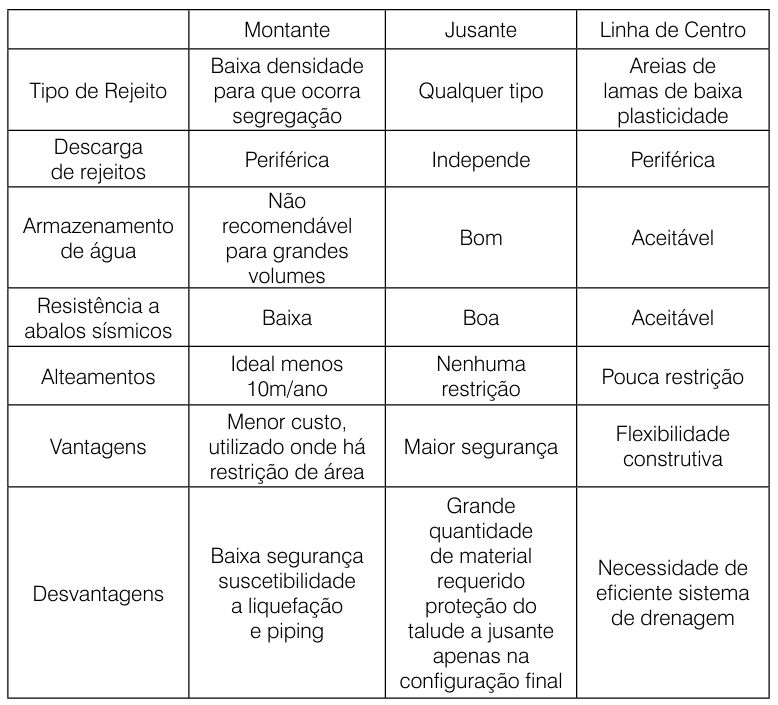
\includegraphics[width=0.9\textwidth]{figures/image18_metodos_construtivos.png}
    \caption{Resumo comparativo dos principais métodos construtivos de barragens de rejeito.}
    \label{fig:metodos_construtivos}
    \fonte{\citeauthor{freire2020rejeitos} (\citeyear{freire2020rejeitos}), p. 110.}
\end{figure}

\subsubsection{Reaproveitamento de rejeitos barragens}
\label{subsubsec:reaproveitamento}

Barragens de rejeitos são reservatórios feitos com o objetivo de reter
água e resíduos sólidos resultantes da extração de minérios para que
evite danos ambientais. (OBTER O TEXTO FINAL - RENATA)

\section{Classificação de risco das barragens de rejeitos}
\label{sec:classificacao_risco}

A mineração no Brasil deu início no século XVII, durante o período
colonial, (OBTER O TEXTO FINAL - RENATA)

\subsection{Risco: Severidade x Probabilidade}
\label{subsec:risco}

Nessa sessão apresenta-se uma visão mineral do Brasil, o papel
fundamental na economia, com impactos significati. (OBTER O TEXTO
FINAL - RENATA)

\section{Legislação ambiental: população e ambiente (Brasil x Exterior)}
\label{sec:legislacao}

No Brasil, a legislação que aborda as barragens de rejeitos,
principalmente as utilizadas na mineração, é bastante detalhada e
abrangente. (OBTER O TEXTO FINAL - RENATA)

\section{Acidentes em Mariana e Brumadinho}
\label{sec:acidentes}

Barragens de rejeitos são reservatórios feitos com o objetivo de reter
água e resíduos sólidos resultantes da extração de minérios para que
evite danos ambientais. (OBTER O TEXTO FINAL - RENATA)

\section{Sistema de alerta existentes}
\label{sec:sistema_alerta}

AQUIIIIII

\subsection{Higrômetro de Resistência e seu uso na prevenção de acidentes de barragens}
\label{subsec:higrometro}
	\chapter{FUNDAMENTAÇÃO TEÓRICA}

Breve descrição do que será apresentado no capítulo. 

< Apresentar os conceitos estudados para desenvolver o trabalho >
	\chapter{MATERIAL E MÉTODOS}\label{cap3MatMet}

< O desenvolvimento é a parte nuclear do trabalho, por vezes denominada
corpo do trabalho. Nessa parte, discute-se o problema apresentado na introdução, bem
como aspectos da metodologia utilizada para a realização do estudo. De acordo com
as características do problema, das técnicas utilizadas e do estilo do autor, pode-se
dividir o desenvolvimento em partes ou capítulos, e cada capítulo em subtítulos ou
itens, sem que se perca a unidade do trabalho. >

Este capítulo aborda as etapas do desenvolvimento do projeto, os materiais
utilizados e a metodologia.

	\chapter{RESULTADOS E DISCUSSÃO}


 \chapter*{}
\noindent
\phantomsection{\MakeUppercase{\textbf{Conclusão e Trabalhos futuros}}}
\addcontentsline{toc}{chapter}{CONCLUSÃO E TRABALHOS FUTUROS}
\vspace{1cm}

Aqui vai a conclusão do trabalho, recapitulando o que foi desenvolvido e os benefícios promovidos pelo que foi desenvolvido no trabalho. 

Em seguida, falar sobre possíveis trabalhos futuros ou continuações do trabalho.

\begin{quote}
\textit{A conclusão proporciona um resumo sintético, mas completo, da argumentação,
das provas consignadas no desenvolvimento do trabalho, como decorrência
natural do que já foi demonstrado. Essa parte deve reunir as características do que
chamamos de síntese interpretativa dos argumentos ou dos elementos contidos no
desenvolvimento do trabalho.}
\end{quote}

\vspace{0.5cm}
\textit{Mais detalhes sobre as regras de construção de uma tese, ver o documento:
roteiro\_uerj\_web.pdf}

    % a abntex2-cite nao aceita o comando \nocite{*}
% portanto cada referencia nao citada deve ser
% adicionada aqui para constar na bibliografia

%\nocite{abnt-classe-doc}

% \nocite{abntex2classe}
% \nocite{abnt-bibtex-doc}
% \nocite{abnt-bibtex-alf-doc}
% \nocite{abnt-classe-doc}
% \nocite{tabela-simbolos-doc}
% \nocite{knuth}
% \nocite{lamport}
% \nocite{lrparsing}
% \nocite{intautomata}
% \nocite{inttheory}
% \nocite{contextfreel}
% \nocite{Kaltofen82factorizationof}
% \nocite{algebramoresym}
% \nocite{elementaryalg}
% \nocite{mathmethods}
% \nocite{symbc}
% \nocite{appliedaero}
% \nocite{cursocalculo}
% \nocite{languagechange}
% \nocite{structureint}
% \nocite{Bartholomew-Biggs2000ADo}
% \nocite{cidoribeiro}
% \nocite{educmat}
% \nocite{useeducation}
% \nocite{precedence}
% \nocite{intautdiff}
% \nocite{autdifftech}
% \nocite{evalderivatives}
% \nocite{modernalgebra}
% \nocite{algalgebra}
    \bibliography{tcc}
	% Elementos pós-textuais
	\postextual
	% \include{glossario}

	%\apendices

\chapter{A experiência de cuidar}
<OPCIONAL>\\
(INFORMAÇÃO ELABORADA PELO PRÓPRIO AUTOR DA MONOGRAFIA)

\chapter{A experiência de estudar}
OPCIONAL\\
(INFORMAÇÃO ELABORADA PELO PRÓPRIO AUTOR DA MONOGRAFIA)

	%\include{anexos} 
	
	
	\appendix

% O algoritmo desenvolvido, na linguagem Python versão 3.7.13, está disponível no seguinte link – \textcolor{blue}{\href{https://colab.research.google.com/drive/15zD5uLvgFG42-VionRbaLIMLS6nAn-d3?usp=sharing}{Predição de casos de COVID-19 em Nova Friburgo}}  – de forma aberta, no Google Colaboratory, para fins de pesquisa e aprofundamento do estudo.
    
\end{document}
